% ****** Start of file aapmsamp.tex ******
%
%   This file is part of the AAPM files in the AAPM distribution for REVTeX 4-2.
%   Version 4.2a of REVTeX, January 2015
%
%   Copyright (c) 2015 American Association of Physicists in Medicine (AAPM).
%
%   See the AAPM README file for restrictions and more information.
%
% TeX'ing this file requires that you have AMS-LaTeX 2.0 installed
% as well as the rest of the prerequisites for REVTeX 4.2
%
% It also requires running BibTeX. The commands are as follows:
%
%  1)  latex  aapmsamp
%  2)  bibtex aapmsamp
%  3)  latex  aapmsamp
%  4)  latex  aapmsamp
%
% Use this file as a source of example code for your aapm document.
% Use the file aapmtemplate.tex as a template for your document.
\documentclass[%
 aapm,
 mph,%
 amsmath,amssymb,
%preprint,%
 reprint,%
%author-year,%
%author-numerical,%
]{revtex4-2}
\usepackage{amssymb}
\usepackage{graphicx}
\usepackage{hyperref}
\usepackage{listings}
\usepackage{mathtools}
\usepackage{booktabs}

\usepackage[table,xcdraw]{xcolor}
% \usepackage{dblfloatfix}

\usepackage{gensymb}
\usepackage{graphicx}% Include figure files
\usepackage{dcolumn}% Align table columns on decimal point
\usepackage{physics}
% \usepackage{mathtools}
% \usepackage{amsmath}
\usepackage{bm}% bold math
\usepackage[mathlines]{lineno}% Enable numbering of text and display math
\usepackage[utf8]{inputenc}
\usepackage[T1]{fontenc}
\usepackage{mathptmx}
\usepackage{etoolbox}

\usepackage{multirow}
\usepackage[normalem]{ulem}
\useunder{\uline}{\ul}{}
\modulolinenumbers[5]% Line numbers with a gap of 5 lines

\begin{document}
\noindent
\header{ENGR 120}
%\preprint{AAPM/123-QED}

\title[]{\underline{Bachelor's Project} \\
Optimizing Atomic Magnetometry with Machine Learning}.% Force line breaks with \\

\author{Christian Emil Lorentsen}%
% \author{Frederik Butler}


\affiliation{Niels Bohr Institute, University of Copenhagen}
\date{\today}% It is always \today, today,
             %  but any date may be explicitly specified
\begin{abstract}
In this report, we use simulated data of a galaxy to train a model which can predict whether a star migrates radially throughout the galaxy, given current measurements of the star. Our focus in this report is prediction, and we will not thoroughly discuss the relationship between the variables and the response.% although we do find that the stars radial component and velocity  are important factors in classifying migrators, due 
We used a wide variety of different models, who were mostly trained on sampled data. The model with the highest accuracy was a fairly simple neural network trained on all of the data, achieving a test accuracy of 88.0\%.
\end{abstract}

\maketitle
\linenumbers\relax % Commence numbering lines
\begin{quotation}
Radial mixing of stars is a crucial dynamical process that we must try to understand if we are to draw significant conclusions about our Galactic history from the properties of stars in our vicinity. Having a model that can accurately predict wether or not a star is a migrator  gains a clearer understanding of the formation, origin of stars and why they are where they are in the galaxy.%, which is crucial in the line of astrophysics.
\end{quotation}


% \section{\label{sec:level1}Background}
% The siphon weir is a relief structure, where when water reaches a certain level, the weir diverts the excess water. 
% \subsection{\label{sec:level2}Theory}
% \input{Chapters/Theory}

\section{\label{sec_level1}Method \& Setup}
The dataset consists of 31 different predictors. These include simulated positions, velocities and atomic ratios of stars inside the milky way. It was generated by R. Roskar, V.P. Debattista,  S.R. Loebman, Z. Ivezic, T.R. Quinn.\cite{Roskar:2011ie}.

To evaluate the performance of different models, we sometimes use cross-entropy, since we have a classification problem. Cross entropy is used to select the best model when performing best subset-selection, although it is not possible to calculate cross-entropy for all of our models, since some do not produce a probability, but classifies wether or not the star is a migrator. To compare all of our models, we use the accuracy\textunderscore score() function from the Python library sklearn.metrcis, where we generally use the cutoff-value of 0.5 for the models, that predict a probability.
% \newpage

\section{DATA AND RESULTS}
\subsection{\label{sec:datasxploration}Data Exploration}
\subsubsection{\label{sec:Matrices}Matrices}

Our first exploration of the dataset, was taking a look at the correlation matrix in table \ref{tab:Correlation} and scatter matrix in figure \ref{fig:scattermatrix} We observe that vx and y are correlated and vy and x are correlated, both at present and at formation. This is due to the fact that the velocity vector is always perpendicular to the position vector in a circular orbit, and therefore when x or y is small, we get high vy and vx. We would get inverted signs for them in our correlation matrix if the orbits were reversed.

We see very strong correlations between the ratios of amounts of atoms in the star. Some of them are very collinear. For example if we look at [O/H] and [MG/H] we see an almost perfect linear relation. In general it seems like all of the scatter plots that plots H as baseline vs H as baseline are very collinear and similarly all scatteplots that plots Fe as baseline vs. Fe as baseline are very collinear. This leads us to believe that there really are only 2 independent variables hidden in all these concentrations i.e. the concentration of iron and the concentration of hydrogen.

We also see the age of the star is strongly correlated with the atomic-concentration fractions. We assume this is due to the star going through different phases of its life and thus changing its chemical composition. 
A similar thing is seen for mass and age where the older the star is the less mass it has. We assume this is due to the fact that stars in general lose mass over their lifetime as a consequence of evaporation and stellar winds, among other things. 

\begin{table*}[t]
\centering
\caption{Correlation matrix of the variables in the dataset}
\label{tab:Correlation}
\resizebox{\textwidth}{!}{
\begin{tabular}{lrrrrrrrrrrrrrrrrrrrrrrrrrrrrrrrr}
\toprule
 & $rsph$ & $x$ & $y$ & $z$ & $vx$ & $vy$ & $vz$ & $Rcyl$ & $\phi$ & $vRcyl$ & $v\phi$ & $rsph_{form}$ & $x_{form}$ & $y_{form}$ & $z_{form}$ & $vx_{form}$ & $vy_{form}$ & $vz_{form}$ & $Rcyl_{form}$ & $\phi_{form}$ & $vRcyl_{form}$ & $v\phi_{form}$ & $age$ & $mass$ & $feh$ & $oh$ & $ch$ & $mgh$ & $ofe$ & $cfe$ & $mgfe$ & $IsMigratorInt$ \\
\midrule
$rsph$ & {\cellcolor[HTML]{081D58}} \color[HTML]{F1F1F1} 1.00 & {\cellcolor[HTML]{F9FDCB}} \color[HTML]{000000} 0.05 & {\cellcolor[HTML]{FFFFD9}} \color[HTML]{000000} -0.02 & {\cellcolor[HTML]{FEFFD6}} \color[HTML]{000000} 0.01 & {\cellcolor[HTML]{F7FCC6}} \color[HTML]{000000} 0.06 & {\cellcolor[HTML]{FFFFD9}} \color[HTML]{000000} -0.00 & {\cellcolor[HTML]{FFFFD9}} \color[HTML]{000000} -0.01 & {\cellcolor[HTML]{081D58}} \color[HTML]{F1F1F1} 1.00 & {\cellcolor[HTML]{FCFED1}} \color[HTML]{000000} 0.02 & {\cellcolor[HTML]{FFFFD9}} \color[HTML]{000000} -0.00 & {\cellcolor[HTML]{B4E2B6}} \color[HTML]{000000} 0.28 & {\cellcolor[HTML]{24479D}} \color[HTML]{F1F1F1} 0.82 & {\cellcolor[HTML]{F3FABF}} \color[HTML]{000000} 0.09 & {\cellcolor[HTML]{FFFFD9}} \color[HTML]{000000} -0.13 & {\cellcolor[HTML]{FCFED3}} \color[HTML]{000000} 0.02 & {\cellcolor[HTML]{FFFFD9}} \color[HTML]{000000} -0.03 & {\cellcolor[HTML]{FFFFD9}} \color[HTML]{000000} -0.02 & {\cellcolor[HTML]{FFFFD9}} \color[HTML]{000000} -0.01 & {\cellcolor[HTML]{24479D}} \color[HTML]{F1F1F1} 0.82 & {\cellcolor[HTML]{F9FDCB}} \color[HTML]{000000} 0.04 & {\cellcolor[HTML]{FFFFD9}} \color[HTML]{000000} -0.01 & {\cellcolor[HTML]{90D4B9}} \color[HTML]{000000} 0.34 & {\cellcolor[HTML]{FFFFD9}} \color[HTML]{000000} -0.35 & {\cellcolor[HTML]{D9F0B3}} \color[HTML]{000000} 0.20 & {\cellcolor[HTML]{EDF8B2}} \color[HTML]{000000} 0.12 & {\cellcolor[HTML]{E8F6B1}} \color[HTML]{000000} 0.14 & {\cellcolor[HTML]{EEF8B3}} \color[HTML]{000000} 0.12 & {\cellcolor[HTML]{ECF7B1}} \color[HTML]{000000} 0.13 & {\cellcolor[HTML]{D1EDB3}} \color[HTML]{000000} 0.22 & {\cellcolor[HTML]{F3FABD}} \color[HTML]{000000} 0.09 & {\cellcolor[HTML]{FFFFD9}} \color[HTML]{000000} -0.05 & {\cellcolor[HTML]{48B9C3}} \color[HTML]{F1F1F1} 0.49 \\
$x$ & {\cellcolor[HTML]{F9FDCB}} \color[HTML]{000000} 0.05 & {\cellcolor[HTML]{081D58}} \color[HTML]{F1F1F1} 1.00 & {\cellcolor[HTML]{FFFFD9}} \color[HTML]{000000} -0.04 & {\cellcolor[HTML]{FFFFD9}} \color[HTML]{000000} 0.00 & {\cellcolor[HTML]{FEFFD6}} \color[HTML]{000000} 0.01 & {\cellcolor[HTML]{36ABC3}} \color[HTML]{F1F1F1} 0.54 & {\cellcolor[HTML]{FFFFD9}} \color[HTML]{000000} -0.00 & {\cellcolor[HTML]{F9FDCB}} \color[HTML]{000000} 0.05 & {\cellcolor[HTML]{FBFDD0}} \color[HTML]{000000} 0.03 & {\cellcolor[HTML]{FEFFD8}} \color[HTML]{000000} 0.01 & {\cellcolor[HTML]{FFFFD9}} \color[HTML]{000000} 0.00 & {\cellcolor[HTML]{FFFFD9}} \color[HTML]{000000} -0.00 & {\cellcolor[HTML]{FCFED3}} \color[HTML]{000000} 0.02 & {\cellcolor[HTML]{FFFFD9}} \color[HTML]{000000} 0.00 & {\cellcolor[HTML]{FFFFD9}} \color[HTML]{000000} -0.00 & {\cellcolor[HTML]{FAFDCF}} \color[HTML]{000000} 0.03 & {\cellcolor[HTML]{FEFFD6}} \color[HTML]{000000} 0.01 & {\cellcolor[HTML]{FFFFD9}} \color[HTML]{000000} -0.00 & {\cellcolor[HTML]{FFFFD9}} \color[HTML]{000000} -0.00 & {\cellcolor[HTML]{FEFFD8}} \color[HTML]{000000} 0.00 & {\cellcolor[HTML]{FFFFD9}} \color[HTML]{000000} -0.01 & {\cellcolor[HTML]{FEFFD6}} \color[HTML]{000000} 0.01 & {\cellcolor[HTML]{FFFFD9}} \color[HTML]{000000} -0.01 & {\cellcolor[HTML]{FFFFD9}} \color[HTML]{000000} 0.00 & {\cellcolor[HTML]{FEFFD8}} \color[HTML]{000000} 0.01 & {\cellcolor[HTML]{FEFFD8}} \color[HTML]{000000} 0.01 & {\cellcolor[HTML]{FEFFD8}} \color[HTML]{000000} 0.01 & {\cellcolor[HTML]{FEFFD8}} \color[HTML]{000000} 0.01 & {\cellcolor[HTML]{FFFFD9}} \color[HTML]{000000} 0.00 & {\cellcolor[HTML]{FFFFD9}} \color[HTML]{000000} 0.00 & {\cellcolor[HTML]{FFFFD9}} \color[HTML]{000000} -0.01 & {\cellcolor[HTML]{FCFED1}} \color[HTML]{000000} 0.03 \\
$y$ & {\cellcolor[HTML]{FFFFD9}} \color[HTML]{000000} -0.02 & {\cellcolor[HTML]{FFFFD9}} \color[HTML]{000000} -0.04 & {\cellcolor[HTML]{081D58}} \color[HTML]{F1F1F1} 1.00 & {\cellcolor[HTML]{FFFFD9}} \color[HTML]{000000} -0.03 & {\cellcolor[HTML]{FFFFD9}} \color[HTML]{000000} -0.55 & {\cellcolor[HTML]{FFFFD9}} \color[HTML]{000000} -0.01 & {\cellcolor[HTML]{FFFFD9}} \color[HTML]{000000} -0.00 & {\cellcolor[HTML]{FFFFD9}} \color[HTML]{000000} -0.02 & {\cellcolor[HTML]{FFFFD9}} \color[HTML]{000000} -0.57 & {\cellcolor[HTML]{FFFFD9}} \color[HTML]{000000} -0.02 & {\cellcolor[HTML]{FFFFD9}} \color[HTML]{000000} -0.02 & {\cellcolor[HTML]{FFFFD9}} \color[HTML]{000000} -0.08 & {\cellcolor[HTML]{FFFFD9}} \color[HTML]{000000} -0.04 & {\cellcolor[HTML]{FFFFD9}} \color[HTML]{000000} -0.02 & {\cellcolor[HTML]{FCFED3}} \color[HTML]{000000} 0.02 & {\cellcolor[HTML]{FCFED3}} \color[HTML]{000000} 0.02 & {\cellcolor[HTML]{FFFFD9}} \color[HTML]{000000} -0.00 & {\cellcolor[HTML]{FFFFD9}} \color[HTML]{000000} -0.00 & {\cellcolor[HTML]{FFFFD9}} \color[HTML]{000000} -0.08 & {\cellcolor[HTML]{FDFED4}} \color[HTML]{000000} 0.02 & {\cellcolor[HTML]{FFFFD9}} \color[HTML]{000000} -0.01 & {\cellcolor[HTML]{FFFFD9}} \color[HTML]{000000} -0.02 & {\cellcolor[HTML]{F9FDCC}} \color[HTML]{000000} 0.04 & {\cellcolor[HTML]{FFFFD9}} \color[HTML]{000000} -0.02 & {\cellcolor[HTML]{FFFFD9}} \color[HTML]{000000} -0.03 & {\cellcolor[HTML]{FFFFD9}} \color[HTML]{000000} -0.03 & {\cellcolor[HTML]{FFFFD9}} \color[HTML]{000000} -0.03 & {\cellcolor[HTML]{FFFFD9}} \color[HTML]{000000} -0.03 & {\cellcolor[HTML]{FFFFD9}} \color[HTML]{000000} -0.01 & {\cellcolor[HTML]{FFFFD9}} \color[HTML]{000000} -0.02 & {\cellcolor[HTML]{FDFED5}} \color[HTML]{000000} 0.01 & {\cellcolor[HTML]{FFFFD9}} \color[HTML]{000000} -0.06 \\
$z$ & {\cellcolor[HTML]{FEFFD6}} \color[HTML]{000000} 0.01 & {\cellcolor[HTML]{FFFFD9}} \color[HTML]{000000} 0.00 & {\cellcolor[HTML]{FFFFD9}} \color[HTML]{000000} -0.03 & {\cellcolor[HTML]{081D58}} \color[HTML]{F1F1F1} 1.00 & {\cellcolor[HTML]{FBFDD0}} \color[HTML]{000000} 0.03 & {\cellcolor[HTML]{FFFFD9}} \color[HTML]{000000} -0.01 & {\cellcolor[HTML]{FFFFD9}} \color[HTML]{000000} -0.01 & {\cellcolor[HTML]{FEFFD8}} \color[HTML]{000000} 0.01 & {\cellcolor[HTML]{FDFED4}} \color[HTML]{000000} 0.02 & {\cellcolor[HTML]{FDFED5}} \color[HTML]{000000} 0.01 & {\cellcolor[HTML]{FCFED3}} \color[HTML]{000000} 0.02 & {\cellcolor[HTML]{FCFED3}} \color[HTML]{000000} 0.02 & {\cellcolor[HTML]{FFFFD9}} \color[HTML]{000000} 0.00 & {\cellcolor[HTML]{FFFFD9}} \color[HTML]{000000} 0.00 & {\cellcolor[HTML]{FEFFD8}} \color[HTML]{000000} 0.00 & {\cellcolor[HTML]{FEFFD8}} \color[HTML]{000000} 0.01 & {\cellcolor[HTML]{FFFFD9}} \color[HTML]{000000} -0.00 & {\cellcolor[HTML]{FFFFD9}} \color[HTML]{000000} -0.01 & {\cellcolor[HTML]{FCFED3}} \color[HTML]{000000} 0.02 & {\cellcolor[HTML]{FFFFD9}} \color[HTML]{000000} -0.01 & {\cellcolor[HTML]{FEFFD6}} \color[HTML]{000000} 0.01 & {\cellcolor[HTML]{FEFFD8}} \color[HTML]{000000} 0.01 & {\cellcolor[HTML]{FFFFD9}} \color[HTML]{000000} -0.00 & {\cellcolor[HTML]{FEFFD8}} \color[HTML]{000000} 0.01 & {\cellcolor[HTML]{FFFFD9}} \color[HTML]{000000} 0.00 & {\cellcolor[HTML]{FFFFD9}} \color[HTML]{000000} 0.00 & {\cellcolor[HTML]{FFFFD9}} \color[HTML]{000000} 0.00 & {\cellcolor[HTML]{FFFFD9}} \color[HTML]{000000} 0.00 & {\cellcolor[HTML]{FFFFD9}} \color[HTML]{000000} 0.00 & {\cellcolor[HTML]{FFFFD9}} \color[HTML]{000000} -0.00 & {\cellcolor[HTML]{FFFFD9}} \color[HTML]{000000} 0.00 & {\cellcolor[HTML]{FCFED3}} \color[HTML]{000000} 0.02 \\
$vx$ & {\cellcolor[HTML]{F7FCC6}} \color[HTML]{000000} 0.06 & {\cellcolor[HTML]{FEFFD6}} \color[HTML]{000000} 0.01 & {\cellcolor[HTML]{FFFFD9}} \color[HTML]{000000} -0.55 & {\cellcolor[HTML]{FBFDD0}} \color[HTML]{000000} 0.03 & {\cellcolor[HTML]{081D58}} \color[HTML]{F1F1F1} 1.00 & {\cellcolor[HTML]{FEFFD8}} \color[HTML]{000000} 0.01 & {\cellcolor[HTML]{FEFFD8}} \color[HTML]{000000} 0.00 & {\cellcolor[HTML]{F7FCC6}} \color[HTML]{000000} 0.06 & {\cellcolor[HTML]{50BBC2}} \color[HTML]{000000} 0.47 & {\cellcolor[HTML]{FDFED5}} \color[HTML]{000000} 0.02 & {\cellcolor[HTML]{FEFFD6}} \color[HTML]{000000} 0.01 & {\cellcolor[HTML]{F3FABD}} \color[HTML]{000000} 0.09 & {\cellcolor[HTML]{FFFFD9}} \color[HTML]{000000} -0.00 & {\cellcolor[HTML]{FEFFD6}} \color[HTML]{000000} 0.01 & {\cellcolor[HTML]{FEFFD6}} \color[HTML]{000000} 0.01 & {\cellcolor[HTML]{FFFFD9}} \color[HTML]{000000} -0.02 & {\cellcolor[HTML]{FFFFD9}} \color[HTML]{000000} -0.02 & {\cellcolor[HTML]{FEFFD8}} \color[HTML]{000000} 0.01 & {\cellcolor[HTML]{F2FABC}} \color[HTML]{000000} 0.09 & {\cellcolor[HTML]{FEFFD6}} \color[HTML]{000000} 0.01 & {\cellcolor[HTML]{FEFFD6}} \color[HTML]{000000} 0.01 & {\cellcolor[HTML]{FCFED3}} \color[HTML]{000000} 0.02 & {\cellcolor[HTML]{FFFFD9}} \color[HTML]{000000} -0.04 & {\cellcolor[HTML]{FCFED3}} \color[HTML]{000000} 0.02 & {\cellcolor[HTML]{FDFED5}} \color[HTML]{000000} 0.01 & {\cellcolor[HTML]{FDFED5}} \color[HTML]{000000} 0.01 & {\cellcolor[HTML]{FEFFD6}} \color[HTML]{000000} 0.01 & {\cellcolor[HTML]{FDFED5}} \color[HTML]{000000} 0.01 & {\cellcolor[HTML]{FEFFD8}} \color[HTML]{000000} 0.01 & {\cellcolor[HTML]{FFFFD9}} \color[HTML]{000000} -0.00 & {\cellcolor[HTML]{FFFFD9}} \color[HTML]{000000} -0.01 & {\cellcolor[HTML]{F6FBC5}} \color[HTML]{000000} 0.07 \\
$vy$ & {\cellcolor[HTML]{FFFFD9}} \color[HTML]{000000} -0.00 & {\cellcolor[HTML]{36ABC3}} \color[HTML]{F1F1F1} 0.54 & {\cellcolor[HTML]{FFFFD9}} \color[HTML]{000000} -0.01 & {\cellcolor[HTML]{FFFFD9}} \color[HTML]{000000} -0.01 & {\cellcolor[HTML]{FEFFD8}} \color[HTML]{000000} 0.01 & {\cellcolor[HTML]{081D58}} \color[HTML]{F1F1F1} 1.00 & {\cellcolor[HTML]{FFFFD9}} \color[HTML]{000000} 0.00 & {\cellcolor[HTML]{FFFFD9}} \color[HTML]{000000} -0.00 & {\cellcolor[HTML]{FFFFD9}} \color[HTML]{000000} 0.00 & {\cellcolor[HTML]{FFFFD9}} \color[HTML]{000000} -0.02 & {\cellcolor[HTML]{FFFFD9}} \color[HTML]{000000} -0.00 & {\cellcolor[HTML]{FFFFD9}} \color[HTML]{000000} -0.03 & {\cellcolor[HTML]{FFFFD9}} \color[HTML]{000000} -0.00 & {\cellcolor[HTML]{FFFFD9}} \color[HTML]{000000} -0.02 & {\cellcolor[HTML]{FFFFD9}} \color[HTML]{000000} 0.00 & {\cellcolor[HTML]{FEFFD6}} \color[HTML]{000000} 0.01 & {\cellcolor[HTML]{FFFFD9}} \color[HTML]{000000} -0.01 & {\cellcolor[HTML]{FFFFD9}} \color[HTML]{000000} 0.00 & {\cellcolor[HTML]{FFFFD9}} \color[HTML]{000000} -0.03 & {\cellcolor[HTML]{FFFFD9}} \color[HTML]{000000} -0.00 & {\cellcolor[HTML]{FDFED5}} \color[HTML]{000000} 0.01 & {\cellcolor[HTML]{FFFFD9}} \color[HTML]{000000} -0.01 & {\cellcolor[HTML]{FDFED4}} \color[HTML]{000000} 0.02 & {\cellcolor[HTML]{FFFFD9}} \color[HTML]{000000} -0.01 & {\cellcolor[HTML]{FFFFD9}} \color[HTML]{000000} -0.01 & {\cellcolor[HTML]{FFFFD9}} \color[HTML]{000000} -0.01 & {\cellcolor[HTML]{FFFFD9}} \color[HTML]{000000} -0.01 & {\cellcolor[HTML]{FFFFD9}} \color[HTML]{000000} -0.01 & {\cellcolor[HTML]{FFFFD9}} \color[HTML]{000000} -0.00 & {\cellcolor[HTML]{FFFFD9}} \color[HTML]{000000} -0.01 & {\cellcolor[HTML]{FEFFD6}} \color[HTML]{000000} 0.01 & {\cellcolor[HTML]{FFFFD9}} \color[HTML]{000000} -0.01 \\
$vz$ & {\cellcolor[HTML]{FFFFD9}} \color[HTML]{000000} -0.01 & {\cellcolor[HTML]{FFFFD9}} \color[HTML]{000000} -0.00 & {\cellcolor[HTML]{FFFFD9}} \color[HTML]{000000} -0.00 & {\cellcolor[HTML]{FFFFD9}} \color[HTML]{000000} -0.01 & {\cellcolor[HTML]{FEFFD8}} \color[HTML]{000000} 0.00 & {\cellcolor[HTML]{FFFFD9}} \color[HTML]{000000} 0.00 & {\cellcolor[HTML]{081D58}} \color[HTML]{F1F1F1} 1.00 & {\cellcolor[HTML]{FFFFD9}} \color[HTML]{000000} -0.01 & {\cellcolor[HTML]{FEFFD8}} \color[HTML]{000000} 0.01 & {\cellcolor[HTML]{FDFED4}} \color[HTML]{000000} 0.02 & {\cellcolor[HTML]{FFFFD9}} \color[HTML]{000000} -0.02 & {\cellcolor[HTML]{FFFFD9}} \color[HTML]{000000} -0.01 & {\cellcolor[HTML]{FEFFD6}} \color[HTML]{000000} 0.01 & {\cellcolor[HTML]{FFFFD9}} \color[HTML]{000000} -0.01 & {\cellcolor[HTML]{FFFFD9}} \color[HTML]{000000} -0.01 & {\cellcolor[HTML]{FFFFD9}} \color[HTML]{000000} -0.01 & {\cellcolor[HTML]{FEFFD6}} \color[HTML]{000000} 0.01 & {\cellcolor[HTML]{FFFFD9}} \color[HTML]{000000} -0.00 & {\cellcolor[HTML]{FFFFD9}} \color[HTML]{000000} -0.01 & {\cellcolor[HTML]{FCFED3}} \color[HTML]{000000} 0.02 & {\cellcolor[HTML]{FFFFD9}} \color[HTML]{000000} -0.01 & {\cellcolor[HTML]{FFFFD9}} \color[HTML]{000000} -0.01 & {\cellcolor[HTML]{FEFFD8}} \color[HTML]{000000} 0.01 & {\cellcolor[HTML]{FFFFD9}} \color[HTML]{000000} -0.01 & {\cellcolor[HTML]{FFFFD9}} \color[HTML]{000000} -0.00 & {\cellcolor[HTML]{FFFFD9}} \color[HTML]{000000} -0.00 & {\cellcolor[HTML]{FFFFD9}} \color[HTML]{000000} -0.00 & {\cellcolor[HTML]{FFFFD9}} \color[HTML]{000000} -0.00 & {\cellcolor[HTML]{FFFFD9}} \color[HTML]{000000} 0.00 & {\cellcolor[HTML]{FFFFD9}} \color[HTML]{000000} 0.00 & {\cellcolor[HTML]{FEFFD8}} \color[HTML]{000000} 0.00 & {\cellcolor[HTML]{FFFFD9}} \color[HTML]{000000} -0.02 \\
$Rcyl$ & {\cellcolor[HTML]{081D58}} \color[HTML]{F1F1F1} 1.00 & {\cellcolor[HTML]{F9FDCB}} \color[HTML]{000000} 0.05 & {\cellcolor[HTML]{FFFFD9}} \color[HTML]{000000} -0.02 & {\cellcolor[HTML]{FEFFD8}} \color[HTML]{000000} 0.01 & {\cellcolor[HTML]{F7FCC6}} \color[HTML]{000000} 0.06 & {\cellcolor[HTML]{FFFFD9}} \color[HTML]{000000} -0.00 & {\cellcolor[HTML]{FFFFD9}} \color[HTML]{000000} -0.01 & {\cellcolor[HTML]{081D58}} \color[HTML]{F1F1F1} 1.00 & {\cellcolor[HTML]{FCFED1}} \color[HTML]{000000} 0.02 & {\cellcolor[HTML]{FFFFD9}} \color[HTML]{000000} -0.00 & {\cellcolor[HTML]{B2E1B6}} \color[HTML]{000000} 0.29 & {\cellcolor[HTML]{24479D}} \color[HTML]{F1F1F1} 0.82 & {\cellcolor[HTML]{F3FABF}} \color[HTML]{000000} 0.09 & {\cellcolor[HTML]{FFFFD9}} \color[HTML]{000000} -0.13 & {\cellcolor[HTML]{FCFED3}} \color[HTML]{000000} 0.02 & {\cellcolor[HTML]{FFFFD9}} \color[HTML]{000000} -0.03 & {\cellcolor[HTML]{FFFFD9}} \color[HTML]{000000} -0.02 & {\cellcolor[HTML]{FFFFD9}} \color[HTML]{000000} -0.01 & {\cellcolor[HTML]{24479D}} \color[HTML]{F1F1F1} 0.82 & {\cellcolor[HTML]{F9FDCC}} \color[HTML]{000000} 0.04 & {\cellcolor[HTML]{FFFFD9}} \color[HTML]{000000} -0.01 & {\cellcolor[HTML]{90D4B9}} \color[HTML]{000000} 0.35 & {\cellcolor[HTML]{FFFFD9}} \color[HTML]{000000} -0.36 & {\cellcolor[HTML]{D7EFB3}} \color[HTML]{000000} 0.20 & {\cellcolor[HTML]{EDF8B1}} \color[HTML]{000000} 0.13 & {\cellcolor[HTML]{E7F6B1}} \color[HTML]{000000} 0.15 & {\cellcolor[HTML]{EDF8B2}} \color[HTML]{000000} 0.12 & {\cellcolor[HTML]{EAF7B1}} \color[HTML]{000000} 0.13 & {\cellcolor[HTML]{D1EDB3}} \color[HTML]{000000} 0.22 & {\cellcolor[HTML]{F2FABC}} \color[HTML]{000000} 0.09 & {\cellcolor[HTML]{FFFFD9}} \color[HTML]{000000} -0.05 & {\cellcolor[HTML]{48B9C3}} \color[HTML]{F1F1F1} 0.49 \\
$\phi$ & {\cellcolor[HTML]{FCFED1}} \color[HTML]{000000} 0.02 & {\cellcolor[HTML]{FBFDD0}} \color[HTML]{000000} 0.03 & {\cellcolor[HTML]{FFFFD9}} \color[HTML]{000000} -0.57 & {\cellcolor[HTML]{FDFED4}} \color[HTML]{000000} 0.02 & {\cellcolor[HTML]{50BBC2}} \color[HTML]{000000} 0.47 & {\cellcolor[HTML]{FFFFD9}} \color[HTML]{000000} 0.00 & {\cellcolor[HTML]{FEFFD8}} \color[HTML]{000000} 0.01 & {\cellcolor[HTML]{FCFED1}} \color[HTML]{000000} 0.02 & {\cellcolor[HTML]{081D58}} \color[HTML]{F1F1F1} 1.00 & {\cellcolor[HTML]{FEFFD8}} \color[HTML]{000000} 0.01 & {\cellcolor[HTML]{FFFFD9}} \color[HTML]{000000} -0.02 & {\cellcolor[HTML]{FAFDCF}} \color[HTML]{000000} 0.03 & {\cellcolor[HTML]{FEFFD8}} \color[HTML]{000000} 0.01 & {\cellcolor[HTML]{FEFFD6}} \color[HTML]{000000} 0.01 & {\cellcolor[HTML]{FFFFD9}} \color[HTML]{000000} -0.01 & {\cellcolor[HTML]{FFFFD9}} \color[HTML]{000000} -0.00 & {\cellcolor[HTML]{FEFFD8}} \color[HTML]{000000} 0.00 & {\cellcolor[HTML]{FFFFD9}} \color[HTML]{000000} 0.00 & {\cellcolor[HTML]{FAFDCE}} \color[HTML]{000000} 0.04 & {\cellcolor[HTML]{FFFFD9}} \color[HTML]{000000} 0.00 & {\cellcolor[HTML]{FDFED4}} \color[HTML]{000000} 0.02 & {\cellcolor[HTML]{FDFED5}} \color[HTML]{000000} 0.01 & {\cellcolor[HTML]{FFFFD9}} \color[HTML]{000000} -0.03 & {\cellcolor[HTML]{FDFED5}} \color[HTML]{000000} 0.01 & {\cellcolor[HTML]{FCFED3}} \color[HTML]{000000} 0.02 & {\cellcolor[HTML]{FCFED3}} \color[HTML]{000000} 0.02 & {\cellcolor[HTML]{FCFED3}} \color[HTML]{000000} 0.02 & {\cellcolor[HTML]{FCFED3}} \color[HTML]{000000} 0.02 & {\cellcolor[HTML]{FFFFD9}} \color[HTML]{000000} -0.00 & {\cellcolor[HTML]{FDFED4}} \color[HTML]{000000} 0.02 & {\cellcolor[HTML]{FFFFD9}} \color[HTML]{000000} -0.02 & {\cellcolor[HTML]{FBFDD0}} \color[HTML]{000000} 0.03 \\
$vRcyl$ & {\cellcolor[HTML]{FFFFD9}} \color[HTML]{000000} -0.00 & {\cellcolor[HTML]{FEFFD8}} \color[HTML]{000000} 0.01 & {\cellcolor[HTML]{FFFFD9}} \color[HTML]{000000} -0.02 & {\cellcolor[HTML]{FDFED5}} \color[HTML]{000000} 0.01 & {\cellcolor[HTML]{FDFED5}} \color[HTML]{000000} 0.02 & {\cellcolor[HTML]{FFFFD9}} \color[HTML]{000000} -0.02 & {\cellcolor[HTML]{FDFED4}} \color[HTML]{000000} 0.02 & {\cellcolor[HTML]{FFFFD9}} \color[HTML]{000000} -0.00 & {\cellcolor[HTML]{FEFFD8}} \color[HTML]{000000} 0.01 & {\cellcolor[HTML]{081D58}} \color[HTML]{F1F1F1} 1.00 & {\cellcolor[HTML]{FEFFD8}} \color[HTML]{000000} 0.00 & {\cellcolor[HTML]{FEFFD6}} \color[HTML]{000000} 0.01 & {\cellcolor[HTML]{FEFFD6}} \color[HTML]{000000} 0.01 & {\cellcolor[HTML]{FFFFD9}} \color[HTML]{000000} -0.00 & {\cellcolor[HTML]{FFFFD9}} \color[HTML]{000000} 0.00 & {\cellcolor[HTML]{FFFFD9}} \color[HTML]{000000} -0.00 & {\cellcolor[HTML]{FFFFD9}} \color[HTML]{000000} 0.00 & {\cellcolor[HTML]{FFFFD9}} \color[HTML]{000000} -0.01 & {\cellcolor[HTML]{FEFFD6}} \color[HTML]{000000} 0.01 & {\cellcolor[HTML]{FEFFD8}} \color[HTML]{000000} 0.01 & {\cellcolor[HTML]{FFFFD9}} \color[HTML]{000000} -0.01 & {\cellcolor[HTML]{FFFFD9}} \color[HTML]{000000} 0.00 & {\cellcolor[HTML]{FFFFD9}} \color[HTML]{000000} -0.00 & {\cellcolor[HTML]{FFFFD9}} \color[HTML]{000000} -0.01 & {\cellcolor[HTML]{FEFFD8}} \color[HTML]{000000} 0.01 & {\cellcolor[HTML]{FEFFD8}} \color[HTML]{000000} 0.01 & {\cellcolor[HTML]{FEFFD8}} \color[HTML]{000000} 0.01 & {\cellcolor[HTML]{FEFFD6}} \color[HTML]{000000} 0.01 & {\cellcolor[HTML]{FFFFD9}} \color[HTML]{000000} -0.01 & {\cellcolor[HTML]{FFFFD9}} \color[HTML]{000000} -0.01 & {\cellcolor[HTML]{FFFFD9}} \color[HTML]{000000} 0.00 & {\cellcolor[HTML]{FFFFD9}} \color[HTML]{000000} 0.00 \\
$v\phi$ & {\cellcolor[HTML]{B4E2B6}} \color[HTML]{000000} 0.28 & {\cellcolor[HTML]{FFFFD9}} \color[HTML]{000000} 0.00 & {\cellcolor[HTML]{FFFFD9}} \color[HTML]{000000} -0.02 & {\cellcolor[HTML]{FCFED3}} \color[HTML]{000000} 0.02 & {\cellcolor[HTML]{FEFFD6}} \color[HTML]{000000} 0.01 & {\cellcolor[HTML]{FFFFD9}} \color[HTML]{000000} -0.00 & {\cellcolor[HTML]{FFFFD9}} \color[HTML]{000000} -0.02 & {\cellcolor[HTML]{B2E1B6}} \color[HTML]{000000} 0.29 & {\cellcolor[HTML]{FFFFD9}} \color[HTML]{000000} -0.02 & {\cellcolor[HTML]{FEFFD8}} \color[HTML]{000000} 0.00 & {\cellcolor[HTML]{081D58}} \color[HTML]{F1F1F1} 1.00 & {\cellcolor[HTML]{92D5B9}} \color[HTML]{000000} 0.34 & {\cellcolor[HTML]{F9FDCB}} \color[HTML]{000000} 0.04 & {\cellcolor[HTML]{FFFFD9}} \color[HTML]{000000} -0.04 & {\cellcolor[HTML]{FDFED4}} \color[HTML]{000000} 0.02 & {\cellcolor[HTML]{FFFFD9}} \color[HTML]{000000} -0.02 & {\cellcolor[HTML]{FEFFD8}} \color[HTML]{000000} 0.01 & {\cellcolor[HTML]{FFFFD9}} \color[HTML]{000000} -0.01 & {\cellcolor[HTML]{87D0BA}} \color[HTML]{000000} 0.36 & {\cellcolor[HTML]{FEFFD6}} \color[HTML]{000000} 0.01 & {\cellcolor[HTML]{FFFFD9}} \color[HTML]{000000} -0.02 & {\cellcolor[HTML]{225EA8}} \color[HTML]{F1F1F1} 0.75 & {\cellcolor[HTML]{FFFFD9}} \color[HTML]{000000} -0.50 & {\cellcolor[HTML]{C4E8B4}} \color[HTML]{000000} 0.26 & {\cellcolor[HTML]{67C4BE}} \color[HTML]{000000} 0.42 & {\cellcolor[HTML]{63C3BF}} \color[HTML]{000000} 0.43 & {\cellcolor[HTML]{69C5BE}} \color[HTML]{000000} 0.42 & {\cellcolor[HTML]{67C4BE}} \color[HTML]{000000} 0.42 & {\cellcolor[HTML]{FBFDD0}} \color[HTML]{000000} 0.03 & {\cellcolor[HTML]{97D6B9}} \color[HTML]{000000} 0.33 & {\cellcolor[HTML]{FFFFD9}} \color[HTML]{000000} -0.31 & {\cellcolor[HTML]{DCF1B2}} \color[HTML]{000000} 0.18 \\
$rsph_{form}$ & {\cellcolor[HTML]{24479D}} \color[HTML]{F1F1F1} 0.82 & {\cellcolor[HTML]{FFFFD9}} \color[HTML]{000000} -0.00 & {\cellcolor[HTML]{FFFFD9}} \color[HTML]{000000} -0.08 & {\cellcolor[HTML]{FCFED3}} \color[HTML]{000000} 0.02 & {\cellcolor[HTML]{F3FABD}} \color[HTML]{000000} 0.09 & {\cellcolor[HTML]{FFFFD9}} \color[HTML]{000000} -0.03 & {\cellcolor[HTML]{FFFFD9}} \color[HTML]{000000} -0.01 & {\cellcolor[HTML]{24479D}} \color[HTML]{F1F1F1} 0.82 & {\cellcolor[HTML]{FAFDCF}} \color[HTML]{000000} 0.03 & {\cellcolor[HTML]{FEFFD6}} \color[HTML]{000000} 0.01 & {\cellcolor[HTML]{92D5B9}} \color[HTML]{000000} 0.34 & {\cellcolor[HTML]{081D58}} \color[HTML]{F1F1F1} 1.00 & {\cellcolor[HTML]{DDF2B2}} \color[HTML]{000000} 0.18 & {\cellcolor[HTML]{FFFFD9}} \color[HTML]{000000} -0.24 & {\cellcolor[HTML]{F9FDCC}} \color[HTML]{000000} 0.04 & {\cellcolor[HTML]{FFFFD9}} \color[HTML]{000000} 0.00 & {\cellcolor[HTML]{FDFED5}} \color[HTML]{000000} 0.01 & {\cellcolor[HTML]{FFFFD9}} \color[HTML]{000000} -0.01 & {\cellcolor[HTML]{091E5A}} \color[HTML]{F1F1F1} 1.00 & {\cellcolor[HTML]{F4FBC0}} \color[HTML]{000000} 0.08 & {\cellcolor[HTML]{FFFFD9}} \color[HTML]{000000} -0.02 & {\cellcolor[HTML]{D6EFB3}} \color[HTML]{000000} 0.20 & {\cellcolor[HTML]{FFFFD9}} \color[HTML]{000000} -0.29 & {\cellcolor[HTML]{E2F4B2}} \color[HTML]{000000} 0.16 & {\cellcolor[HTML]{F5FBC4}} \color[HTML]{000000} 0.07 & {\cellcolor[HTML]{F3FABD}} \color[HTML]{000000} 0.09 & {\cellcolor[HTML]{F5FBC4}} \color[HTML]{000000} 0.07 & {\cellcolor[HTML]{F4FBC1}} \color[HTML]{000000} 0.08 & {\cellcolor[HTML]{D4EEB3}} \color[HTML]{000000} 0.21 & {\cellcolor[HTML]{F9FDCB}} \color[HTML]{000000} 0.04 & {\cellcolor[HTML]{FFFFD9}} \color[HTML]{000000} -0.01 & {\cellcolor[HTML]{2FA4C2}} \color[HTML]{F1F1F1} 0.56 \\
$x_{form}$ & {\cellcolor[HTML]{F3FABF}} \color[HTML]{000000} 0.09 & {\cellcolor[HTML]{FCFED3}} \color[HTML]{000000} 0.02 & {\cellcolor[HTML]{FFFFD9}} \color[HTML]{000000} -0.04 & {\cellcolor[HTML]{FFFFD9}} \color[HTML]{000000} 0.00 & {\cellcolor[HTML]{FFFFD9}} \color[HTML]{000000} -0.00 & {\cellcolor[HTML]{FFFFD9}} \color[HTML]{000000} -0.00 & {\cellcolor[HTML]{FEFFD6}} \color[HTML]{000000} 0.01 & {\cellcolor[HTML]{F3FABF}} \color[HTML]{000000} 0.09 & {\cellcolor[HTML]{FEFFD8}} \color[HTML]{000000} 0.01 & {\cellcolor[HTML]{FEFFD6}} \color[HTML]{000000} 0.01 & {\cellcolor[HTML]{F9FDCB}} \color[HTML]{000000} 0.04 & {\cellcolor[HTML]{DDF2B2}} \color[HTML]{000000} 0.18 & {\cellcolor[HTML]{081D58}} \color[HTML]{F1F1F1} 1.00 & {\cellcolor[HTML]{FFFFD9}} \color[HTML]{000000} -0.11 & {\cellcolor[HTML]{FEFFD6}} \color[HTML]{000000} 0.01 & {\cellcolor[HTML]{FCFED3}} \color[HTML]{000000} 0.02 & {\cellcolor[HTML]{3DB2C4}} \color[HTML]{F1F1F1} 0.51 & {\cellcolor[HTML]{FFFFD9}} \color[HTML]{000000} -0.01 & {\cellcolor[HTML]{DDF2B2}} \color[HTML]{000000} 0.18 & {\cellcolor[HTML]{F8FCC9}} \color[HTML]{000000} 0.05 & {\cellcolor[HTML]{FFFFD9}} \color[HTML]{000000} -0.04 & {\cellcolor[HTML]{FFFFD9}} \color[HTML]{000000} 0.00 & {\cellcolor[HTML]{FFFFD9}} \color[HTML]{000000} -0.04 & {\cellcolor[HTML]{FBFDD0}} \color[HTML]{000000} 0.03 & {\cellcolor[HTML]{FCFED1}} \color[HTML]{000000} 0.02 & {\cellcolor[HTML]{FCFED1}} \color[HTML]{000000} 0.03 & {\cellcolor[HTML]{FCFED3}} \color[HTML]{000000} 0.02 & {\cellcolor[HTML]{FCFED1}} \color[HTML]{000000} 0.03 & {\cellcolor[HTML]{FDFED5}} \color[HTML]{000000} 0.01 & {\cellcolor[HTML]{FEFFD6}} \color[HTML]{000000} 0.01 & {\cellcolor[HTML]{FFFFD9}} \color[HTML]{000000} -0.01 & {\cellcolor[HTML]{EFF9B6}} \color[HTML]{000000} 0.11 \\
$y_{form}$ & {\cellcolor[HTML]{FFFFD9}} \color[HTML]{000000} -0.13 & {\cellcolor[HTML]{FFFFD9}} \color[HTML]{000000} 0.00 & {\cellcolor[HTML]{FFFFD9}} \color[HTML]{000000} -0.02 & {\cellcolor[HTML]{FFFFD9}} \color[HTML]{000000} 0.00 & {\cellcolor[HTML]{FEFFD6}} \color[HTML]{000000} 0.01 & {\cellcolor[HTML]{FFFFD9}} \color[HTML]{000000} -0.02 & {\cellcolor[HTML]{FFFFD9}} \color[HTML]{000000} -0.01 & {\cellcolor[HTML]{FFFFD9}} \color[HTML]{000000} -0.13 & {\cellcolor[HTML]{FEFFD6}} \color[HTML]{000000} 0.01 & {\cellcolor[HTML]{FFFFD9}} \color[HTML]{000000} -0.00 & {\cellcolor[HTML]{FFFFD9}} \color[HTML]{000000} -0.04 & {\cellcolor[HTML]{FFFFD9}} \color[HTML]{000000} -0.24 & {\cellcolor[HTML]{FFFFD9}} \color[HTML]{000000} -0.11 & {\cellcolor[HTML]{081D58}} \color[HTML]{F1F1F1} 1.00 & {\cellcolor[HTML]{FFFFD9}} \color[HTML]{000000} -0.03 & {\cellcolor[HTML]{FFFFD9}} \color[HTML]{000000} -0.50 & {\cellcolor[HTML]{FFFFD9}} \color[HTML]{000000} -0.03 & {\cellcolor[HTML]{FFFFD9}} \color[HTML]{000000} -0.00 & {\cellcolor[HTML]{FFFFD9}} \color[HTML]{000000} -0.24 & {\cellcolor[HTML]{FFFFD9}} \color[HTML]{000000} -0.54 & {\cellcolor[HTML]{FFFFD9}} \color[HTML]{000000} -0.02 & {\cellcolor[HTML]{FFFFD9}} \color[HTML]{000000} -0.02 & {\cellcolor[HTML]{F7FCC7}} \color[HTML]{000000} 0.06 & {\cellcolor[HTML]{FFFFD9}} \color[HTML]{000000} -0.04 & {\cellcolor[HTML]{FFFFD9}} \color[HTML]{000000} -0.02 & {\cellcolor[HTML]{FFFFD9}} \color[HTML]{000000} -0.02 & {\cellcolor[HTML]{FFFFD9}} \color[HTML]{000000} -0.02 & {\cellcolor[HTML]{FFFFD9}} \color[HTML]{000000} -0.02 & {\cellcolor[HTML]{FFFFD9}} \color[HTML]{000000} -0.02 & {\cellcolor[HTML]{FFFFD9}} \color[HTML]{000000} -0.02 & {\cellcolor[HTML]{FDFED4}} \color[HTML]{000000} 0.02 & {\cellcolor[HTML]{FFFFD9}} \color[HTML]{000000} -0.11 \\
$z_{form}$ & {\cellcolor[HTML]{FCFED3}} \color[HTML]{000000} 0.02 & {\cellcolor[HTML]{FFFFD9}} \color[HTML]{000000} -0.00 & {\cellcolor[HTML]{FCFED3}} \color[HTML]{000000} 0.02 & {\cellcolor[HTML]{FEFFD8}} \color[HTML]{000000} 0.00 & {\cellcolor[HTML]{FEFFD6}} \color[HTML]{000000} 0.01 & {\cellcolor[HTML]{FFFFD9}} \color[HTML]{000000} 0.00 & {\cellcolor[HTML]{FFFFD9}} \color[HTML]{000000} -0.01 & {\cellcolor[HTML]{FCFED3}} \color[HTML]{000000} 0.02 & {\cellcolor[HTML]{FFFFD9}} \color[HTML]{000000} -0.01 & {\cellcolor[HTML]{FFFFD9}} \color[HTML]{000000} 0.00 & {\cellcolor[HTML]{FDFED4}} \color[HTML]{000000} 0.02 & {\cellcolor[HTML]{F9FDCC}} \color[HTML]{000000} 0.04 & {\cellcolor[HTML]{FEFFD6}} \color[HTML]{000000} 0.01 & {\cellcolor[HTML]{FFFFD9}} \color[HTML]{000000} -0.03 & {\cellcolor[HTML]{081D58}} \color[HTML]{F1F1F1} 1.00 & {\cellcolor[HTML]{FEFFD6}} \color[HTML]{000000} 0.01 & {\cellcolor[HTML]{FFFFD9}} \color[HTML]{000000} 0.00 & {\cellcolor[HTML]{FEFFD6}} \color[HTML]{000000} 0.01 & {\cellcolor[HTML]{FAFDCE}} \color[HTML]{000000} 0.04 & {\cellcolor[HTML]{FDFED4}} \color[HTML]{000000} 0.02 & {\cellcolor[HTML]{FEFFD6}} \color[HTML]{000000} 0.01 & {\cellcolor[HTML]{FDFED5}} \color[HTML]{000000} 0.01 & {\cellcolor[HTML]{FFFFD9}} \color[HTML]{000000} -0.02 & {\cellcolor[HTML]{FDFED5}} \color[HTML]{000000} 0.01 & {\cellcolor[HTML]{FEFFD6}} \color[HTML]{000000} 0.01 & {\cellcolor[HTML]{FEFFD6}} \color[HTML]{000000} 0.01 & {\cellcolor[HTML]{FEFFD6}} \color[HTML]{000000} 0.01 & {\cellcolor[HTML]{FEFFD6}} \color[HTML]{000000} 0.01 & {\cellcolor[HTML]{FFFFD9}} \color[HTML]{000000} -0.00 & {\cellcolor[HTML]{FEFFD8}} \color[HTML]{000000} 0.01 & {\cellcolor[HTML]{FFFFD9}} \color[HTML]{000000} -0.01 & {\cellcolor[HTML]{FCFED1}} \color[HTML]{000000} 0.03 \\
$vx_{form}$ & {\cellcolor[HTML]{FFFFD9}} \color[HTML]{000000} -0.03 & {\cellcolor[HTML]{FAFDCF}} \color[HTML]{000000} 0.03 & {\cellcolor[HTML]{FCFED3}} \color[HTML]{000000} 0.02 & {\cellcolor[HTML]{FEFFD8}} \color[HTML]{000000} 0.01 & {\cellcolor[HTML]{FFFFD9}} \color[HTML]{000000} -0.02 & {\cellcolor[HTML]{FEFFD6}} \color[HTML]{000000} 0.01 & {\cellcolor[HTML]{FFFFD9}} \color[HTML]{000000} -0.01 & {\cellcolor[HTML]{FFFFD9}} \color[HTML]{000000} -0.03 & {\cellcolor[HTML]{FFFFD9}} \color[HTML]{000000} -0.00 & {\cellcolor[HTML]{FFFFD9}} \color[HTML]{000000} -0.00 & {\cellcolor[HTML]{FFFFD9}} \color[HTML]{000000} -0.02 & {\cellcolor[HTML]{FFFFD9}} \color[HTML]{000000} 0.00 & {\cellcolor[HTML]{FCFED3}} \color[HTML]{000000} 0.02 & {\cellcolor[HTML]{FFFFD9}} \color[HTML]{000000} -0.50 & {\cellcolor[HTML]{FEFFD6}} \color[HTML]{000000} 0.01 & {\cellcolor[HTML]{081D58}} \color[HTML]{F1F1F1} 1.00 & {\cellcolor[HTML]{FAFDCE}} \color[HTML]{000000} 0.04 & {\cellcolor[HTML]{FFFFD9}} \color[HTML]{000000} -0.01 & {\cellcolor[HTML]{FFFFD9}} \color[HTML]{000000} 0.00 & {\cellcolor[HTML]{55BEC1}} \color[HTML]{000000} 0.46 & {\cellcolor[HTML]{FAFDCE}} \color[HTML]{000000} 0.04 & {\cellcolor[HTML]{FFFFD9}} \color[HTML]{000000} -0.00 & {\cellcolor[HTML]{FFFFD9}} \color[HTML]{000000} -0.00 & {\cellcolor[HTML]{FFFFD9}} \color[HTML]{000000} -0.00 & {\cellcolor[HTML]{FEFFD8}} \color[HTML]{000000} 0.00 & {\cellcolor[HTML]{FEFFD8}} \color[HTML]{000000} 0.00 & {\cellcolor[HTML]{FEFFD8}} \color[HTML]{000000} 0.01 & {\cellcolor[HTML]{FEFFD8}} \color[HTML]{000000} 0.00 & {\cellcolor[HTML]{FEFFD8}} \color[HTML]{000000} 0.01 & {\cellcolor[HTML]{FEFFD6}} \color[HTML]{000000} 0.01 & {\cellcolor[HTML]{FFFFD9}} \color[HTML]{000000} -0.00 & {\cellcolor[HTML]{FFFFD9}} \color[HTML]{000000} -0.02 \\
$vy_{form}$ & {\cellcolor[HTML]{FFFFD9}} \color[HTML]{000000} -0.02 & {\cellcolor[HTML]{FEFFD6}} \color[HTML]{000000} 0.01 & {\cellcolor[HTML]{FFFFD9}} \color[HTML]{000000} -0.00 & {\cellcolor[HTML]{FFFFD9}} \color[HTML]{000000} -0.00 & {\cellcolor[HTML]{FFFFD9}} \color[HTML]{000000} -0.02 & {\cellcolor[HTML]{FFFFD9}} \color[HTML]{000000} -0.01 & {\cellcolor[HTML]{FEFFD6}} \color[HTML]{000000} 0.01 & {\cellcolor[HTML]{FFFFD9}} \color[HTML]{000000} -0.02 & {\cellcolor[HTML]{FEFFD8}} \color[HTML]{000000} 0.00 & {\cellcolor[HTML]{FFFFD9}} \color[HTML]{000000} 0.00 & {\cellcolor[HTML]{FEFFD8}} \color[HTML]{000000} 0.01 & {\cellcolor[HTML]{FDFED5}} \color[HTML]{000000} 0.01 & {\cellcolor[HTML]{3DB2C4}} \color[HTML]{F1F1F1} 0.51 & {\cellcolor[HTML]{FFFFD9}} \color[HTML]{000000} -0.03 & {\cellcolor[HTML]{FFFFD9}} \color[HTML]{000000} 0.00 & {\cellcolor[HTML]{FAFDCE}} \color[HTML]{000000} 0.04 & {\cellcolor[HTML]{081D58}} \color[HTML]{F1F1F1} 1.00 & {\cellcolor[HTML]{FFFFD9}} \color[HTML]{000000} -0.03 & {\cellcolor[HTML]{FEFFD6}} \color[HTML]{000000} 0.01 & {\cellcolor[HTML]{FEFFD6}} \color[HTML]{000000} 0.01 & {\cellcolor[HTML]{FFFFD9}} \color[HTML]{000000} 0.00 & {\cellcolor[HTML]{FFFFD9}} \color[HTML]{000000} -0.00 & {\cellcolor[HTML]{FDFED4}} \color[HTML]{000000} 0.02 & {\cellcolor[HTML]{FFFFD9}} \color[HTML]{000000} -0.01 & {\cellcolor[HTML]{FFFFD9}} \color[HTML]{000000} -0.01 & {\cellcolor[HTML]{FFFFD9}} \color[HTML]{000000} -0.01 & {\cellcolor[HTML]{FFFFD9}} \color[HTML]{000000} -0.01 & {\cellcolor[HTML]{FFFFD9}} \color[HTML]{000000} -0.01 & {\cellcolor[HTML]{FDFED4}} \color[HTML]{000000} 0.02 & {\cellcolor[HTML]{FFFFD9}} \color[HTML]{000000} -0.01 & {\cellcolor[HTML]{FDFED5}} \color[HTML]{000000} 0.01 & {\cellcolor[HTML]{FEFFD6}} \color[HTML]{000000} 0.01 \\
$vz_{form}$ & {\cellcolor[HTML]{FFFFD9}} \color[HTML]{000000} -0.01 & {\cellcolor[HTML]{FFFFD9}} \color[HTML]{000000} -0.00 & {\cellcolor[HTML]{FFFFD9}} \color[HTML]{000000} -0.00 & {\cellcolor[HTML]{FFFFD9}} \color[HTML]{000000} -0.01 & {\cellcolor[HTML]{FEFFD8}} \color[HTML]{000000} 0.01 & {\cellcolor[HTML]{FFFFD9}} \color[HTML]{000000} 0.00 & {\cellcolor[HTML]{FFFFD9}} \color[HTML]{000000} -0.00 & {\cellcolor[HTML]{FFFFD9}} \color[HTML]{000000} -0.01 & {\cellcolor[HTML]{FFFFD9}} \color[HTML]{000000} 0.00 & {\cellcolor[HTML]{FFFFD9}} \color[HTML]{000000} -0.01 & {\cellcolor[HTML]{FFFFD9}} \color[HTML]{000000} -0.01 & {\cellcolor[HTML]{FFFFD9}} \color[HTML]{000000} -0.01 & {\cellcolor[HTML]{FFFFD9}} \color[HTML]{000000} -0.01 & {\cellcolor[HTML]{FFFFD9}} \color[HTML]{000000} -0.00 & {\cellcolor[HTML]{FEFFD6}} \color[HTML]{000000} 0.01 & {\cellcolor[HTML]{FFFFD9}} \color[HTML]{000000} -0.01 & {\cellcolor[HTML]{FFFFD9}} \color[HTML]{000000} -0.03 & {\cellcolor[HTML]{081D58}} \color[HTML]{F1F1F1} 1.00 & {\cellcolor[HTML]{FFFFD9}} \color[HTML]{000000} -0.01 & {\cellcolor[HTML]{FFFFD9}} \color[HTML]{000000} -0.01 & {\cellcolor[HTML]{FFFFD9}} \color[HTML]{000000} 0.00 & {\cellcolor[HTML]{FFFFD9}} \color[HTML]{000000} -0.00 & {\cellcolor[HTML]{FEFFD6}} \color[HTML]{000000} 0.01 & {\cellcolor[HTML]{FFFFD9}} \color[HTML]{000000} -0.00 & {\cellcolor[HTML]{FFFFD9}} \color[HTML]{000000} -0.01 & {\cellcolor[HTML]{FFFFD9}} \color[HTML]{000000} -0.01 & {\cellcolor[HTML]{FFFFD9}} \color[HTML]{000000} -0.01 & {\cellcolor[HTML]{FFFFD9}} \color[HTML]{000000} -0.01 & {\cellcolor[HTML]{FFFFD9}} \color[HTML]{000000} -0.00 & {\cellcolor[HTML]{FFFFD9}} \color[HTML]{000000} -0.01 & {\cellcolor[HTML]{FEFFD6}} \color[HTML]{000000} 0.01 & {\cellcolor[HTML]{FFFFD9}} \color[HTML]{000000} 0.00 \\
$Rcyl_{form}$ & {\cellcolor[HTML]{24479D}} \color[HTML]{F1F1F1} 0.82 & {\cellcolor[HTML]{FFFFD9}} \color[HTML]{000000} -0.00 & {\cellcolor[HTML]{FFFFD9}} \color[HTML]{000000} -0.08 & {\cellcolor[HTML]{FCFED3}} \color[HTML]{000000} 0.02 & {\cellcolor[HTML]{F2FABC}} \color[HTML]{000000} 0.09 & {\cellcolor[HTML]{FFFFD9}} \color[HTML]{000000} -0.03 & {\cellcolor[HTML]{FFFFD9}} \color[HTML]{000000} -0.01 & {\cellcolor[HTML]{24479D}} \color[HTML]{F1F1F1} 0.82 & {\cellcolor[HTML]{FAFDCE}} \color[HTML]{000000} 0.04 & {\cellcolor[HTML]{FEFFD6}} \color[HTML]{000000} 0.01 & {\cellcolor[HTML]{87D0BA}} \color[HTML]{000000} 0.36 & {\cellcolor[HTML]{091E5A}} \color[HTML]{F1F1F1} 1.00 & {\cellcolor[HTML]{DDF2B2}} \color[HTML]{000000} 0.18 & {\cellcolor[HTML]{FFFFD9}} \color[HTML]{000000} -0.24 & {\cellcolor[HTML]{FAFDCE}} \color[HTML]{000000} 0.04 & {\cellcolor[HTML]{FFFFD9}} \color[HTML]{000000} 0.00 & {\cellcolor[HTML]{FEFFD6}} \color[HTML]{000000} 0.01 & {\cellcolor[HTML]{FFFFD9}} \color[HTML]{000000} -0.01 & {\cellcolor[HTML]{081D58}} \color[HTML]{F1F1F1} 1.00 & {\cellcolor[HTML]{F4FBC0}} \color[HTML]{000000} 0.08 & {\cellcolor[HTML]{FFFFD9}} \color[HTML]{000000} -0.02 & {\cellcolor[HTML]{D0EDB3}} \color[HTML]{000000} 0.22 & {\cellcolor[HTML]{FFFFD9}} \color[HTML]{000000} -0.32 & {\cellcolor[HTML]{DFF2B2}} \color[HTML]{000000} 0.17 & {\cellcolor[HTML]{F1FABA}} \color[HTML]{000000} 0.10 & {\cellcolor[HTML]{EFF9B5}} \color[HTML]{000000} 0.12 & {\cellcolor[HTML]{F1FABB}} \color[HTML]{000000} 0.10 & {\cellcolor[HTML]{F0F9B8}} \color[HTML]{000000} 0.10 & {\cellcolor[HTML]{D6EFB3}} \color[HTML]{000000} 0.20 & {\cellcolor[HTML]{F5FBC4}} \color[HTML]{000000} 0.07 & {\cellcolor[HTML]{FFFFD9}} \color[HTML]{000000} -0.03 & {\cellcolor[HTML]{31A5C2}} \color[HTML]{F1F1F1} 0.55 \\
$\phi_{form}$ & {\cellcolor[HTML]{F9FDCB}} \color[HTML]{000000} 0.04 & {\cellcolor[HTML]{FEFFD8}} \color[HTML]{000000} 0.00 & {\cellcolor[HTML]{FDFED4}} \color[HTML]{000000} 0.02 & {\cellcolor[HTML]{FFFFD9}} \color[HTML]{000000} -0.01 & {\cellcolor[HTML]{FEFFD6}} \color[HTML]{000000} 0.01 & {\cellcolor[HTML]{FFFFD9}} \color[HTML]{000000} -0.00 & {\cellcolor[HTML]{FCFED3}} \color[HTML]{000000} 0.02 & {\cellcolor[HTML]{F9FDCC}} \color[HTML]{000000} 0.04 & {\cellcolor[HTML]{FFFFD9}} \color[HTML]{000000} 0.00 & {\cellcolor[HTML]{FEFFD8}} \color[HTML]{000000} 0.01 & {\cellcolor[HTML]{FEFFD6}} \color[HTML]{000000} 0.01 & {\cellcolor[HTML]{F4FBC0}} \color[HTML]{000000} 0.08 & {\cellcolor[HTML]{F8FCC9}} \color[HTML]{000000} 0.05 & {\cellcolor[HTML]{FFFFD9}} \color[HTML]{000000} -0.54 & {\cellcolor[HTML]{FDFED4}} \color[HTML]{000000} 0.02 & {\cellcolor[HTML]{55BEC1}} \color[HTML]{000000} 0.46 & {\cellcolor[HTML]{FEFFD6}} \color[HTML]{000000} 0.01 & {\cellcolor[HTML]{FFFFD9}} \color[HTML]{000000} -0.01 & {\cellcolor[HTML]{F4FBC0}} \color[HTML]{000000} 0.08 & {\cellcolor[HTML]{081D58}} \color[HTML]{F1F1F1} 1.00 & {\cellcolor[HTML]{FFFFD9}} \color[HTML]{000000} 0.00 & {\cellcolor[HTML]{FAFDCF}} \color[HTML]{000000} 0.03 & {\cellcolor[HTML]{FFFFD9}} \color[HTML]{000000} -0.03 & {\cellcolor[HTML]{FDFED5}} \color[HTML]{000000} 0.02 & {\cellcolor[HTML]{FDFED5}} \color[HTML]{000000} 0.01 & {\cellcolor[HTML]{FDFED5}} \color[HTML]{000000} 0.01 & {\cellcolor[HTML]{FDFED5}} \color[HTML]{000000} 0.01 & {\cellcolor[HTML]{FDFED5}} \color[HTML]{000000} 0.01 & {\cellcolor[HTML]{FFFFD9}} \color[HTML]{000000} 0.00 & {\cellcolor[HTML]{FCFED3}} \color[HTML]{000000} 0.02 & {\cellcolor[HTML]{FFFFD9}} \color[HTML]{000000} -0.01 & {\cellcolor[HTML]{F9FDCC}} \color[HTML]{000000} 0.04 \\
$vRcyl_{form}$ & {\cellcolor[HTML]{FFFFD9}} \color[HTML]{000000} -0.01 & {\cellcolor[HTML]{FFFFD9}} \color[HTML]{000000} -0.01 & {\cellcolor[HTML]{FFFFD9}} \color[HTML]{000000} -0.01 & {\cellcolor[HTML]{FEFFD6}} \color[HTML]{000000} 0.01 & {\cellcolor[HTML]{FEFFD6}} \color[HTML]{000000} 0.01 & {\cellcolor[HTML]{FDFED5}} \color[HTML]{000000} 0.01 & {\cellcolor[HTML]{FFFFD9}} \color[HTML]{000000} -0.01 & {\cellcolor[HTML]{FFFFD9}} \color[HTML]{000000} -0.01 & {\cellcolor[HTML]{FDFED4}} \color[HTML]{000000} 0.02 & {\cellcolor[HTML]{FFFFD9}} \color[HTML]{000000} -0.01 & {\cellcolor[HTML]{FFFFD9}} \color[HTML]{000000} -0.02 & {\cellcolor[HTML]{FFFFD9}} \color[HTML]{000000} -0.02 & {\cellcolor[HTML]{FFFFD9}} \color[HTML]{000000} -0.04 & {\cellcolor[HTML]{FFFFD9}} \color[HTML]{000000} -0.02 & {\cellcolor[HTML]{FEFFD6}} \color[HTML]{000000} 0.01 & {\cellcolor[HTML]{FAFDCE}} \color[HTML]{000000} 0.04 & {\cellcolor[HTML]{FFFFD9}} \color[HTML]{000000} 0.00 & {\cellcolor[HTML]{FFFFD9}} \color[HTML]{000000} 0.00 & {\cellcolor[HTML]{FFFFD9}} \color[HTML]{000000} -0.02 & {\cellcolor[HTML]{FFFFD9}} \color[HTML]{000000} 0.00 & {\cellcolor[HTML]{081D58}} \color[HTML]{F1F1F1} 1.00 & {\cellcolor[HTML]{FFFFD9}} \color[HTML]{000000} -0.00 & {\cellcolor[HTML]{FFFFD9}} \color[HTML]{000000} 0.00 & {\cellcolor[HTML]{FFFFD9}} \color[HTML]{000000} 0.00 & {\cellcolor[HTML]{FFFFD9}} \color[HTML]{000000} 0.00 & {\cellcolor[HTML]{FFFFD9}} \color[HTML]{000000} 0.00 & {\cellcolor[HTML]{FFFFD9}} \color[HTML]{000000} 0.00 & {\cellcolor[HTML]{FFFFD9}} \color[HTML]{000000} 0.00 & {\cellcolor[HTML]{FFFFD9}} \color[HTML]{000000} -0.02 & {\cellcolor[HTML]{FEFFD8}} \color[HTML]{000000} 0.01 & {\cellcolor[HTML]{FFFFD9}} \color[HTML]{000000} -0.01 & {\cellcolor[HTML]{FFFFD9}} \color[HTML]{000000} 0.00 \\
$v\phi_{form}$ & {\cellcolor[HTML]{90D4B9}} \color[HTML]{000000} 0.34 & {\cellcolor[HTML]{FEFFD6}} \color[HTML]{000000} 0.01 & {\cellcolor[HTML]{FFFFD9}} \color[HTML]{000000} -0.02 & {\cellcolor[HTML]{FEFFD8}} \color[HTML]{000000} 0.01 & {\cellcolor[HTML]{FCFED3}} \color[HTML]{000000} 0.02 & {\cellcolor[HTML]{FFFFD9}} \color[HTML]{000000} -0.01 & {\cellcolor[HTML]{FFFFD9}} \color[HTML]{000000} -0.01 & {\cellcolor[HTML]{90D4B9}} \color[HTML]{000000} 0.35 & {\cellcolor[HTML]{FDFED5}} \color[HTML]{000000} 0.01 & {\cellcolor[HTML]{FFFFD9}} \color[HTML]{000000} 0.00 & {\cellcolor[HTML]{225EA8}} \color[HTML]{F1F1F1} 0.75 & {\cellcolor[HTML]{D6EFB3}} \color[HTML]{000000} 0.20 & {\cellcolor[HTML]{FFFFD9}} \color[HTML]{000000} 0.00 & {\cellcolor[HTML]{FFFFD9}} \color[HTML]{000000} -0.02 & {\cellcolor[HTML]{FDFED5}} \color[HTML]{000000} 0.01 & {\cellcolor[HTML]{FFFFD9}} \color[HTML]{000000} -0.00 & {\cellcolor[HTML]{FFFFD9}} \color[HTML]{000000} -0.00 & {\cellcolor[HTML]{FFFFD9}} \color[HTML]{000000} -0.00 & {\cellcolor[HTML]{D0EDB3}} \color[HTML]{000000} 0.22 & {\cellcolor[HTML]{FAFDCF}} \color[HTML]{000000} 0.03 & {\cellcolor[HTML]{FFFFD9}} \color[HTML]{000000} -0.00 & {\cellcolor[HTML]{081D58}} \color[HTML]{F1F1F1} 1.00 & {\cellcolor[HTML]{FFFFD9}} \color[HTML]{000000} -0.52 & {\cellcolor[HTML]{BBE4B5}} \color[HTML]{000000} 0.27 & {\cellcolor[HTML]{5DC0C0}} \color[HTML]{000000} 0.44 & {\cellcolor[HTML]{59BFC0}} \color[HTML]{000000} 0.45 & {\cellcolor[HTML]{5FC1C0}} \color[HTML]{000000} 0.44 & {\cellcolor[HTML]{5BC0C0}} \color[HTML]{000000} 0.45 & {\cellcolor[HTML]{FCFED3}} \color[HTML]{000000} 0.02 & {\cellcolor[HTML]{8CD2BA}} \color[HTML]{000000} 0.35 & {\cellcolor[HTML]{FFFFD9}} \color[HTML]{000000} -0.33 & {\cellcolor[HTML]{EFF9B5}} \color[HTML]{000000} 0.11 \\
$age$ & {\cellcolor[HTML]{FFFFD9}} \color[HTML]{000000} -0.35 & {\cellcolor[HTML]{FFFFD9}} \color[HTML]{000000} -0.01 & {\cellcolor[HTML]{F9FDCC}} \color[HTML]{000000} 0.04 & {\cellcolor[HTML]{FFFFD9}} \color[HTML]{000000} -0.00 & {\cellcolor[HTML]{FFFFD9}} \color[HTML]{000000} -0.04 & {\cellcolor[HTML]{FDFED4}} \color[HTML]{000000} 0.02 & {\cellcolor[HTML]{FEFFD8}} \color[HTML]{000000} 0.01 & {\cellcolor[HTML]{FFFFD9}} \color[HTML]{000000} -0.36 & {\cellcolor[HTML]{FFFFD9}} \color[HTML]{000000} -0.03 & {\cellcolor[HTML]{FFFFD9}} \color[HTML]{000000} -0.00 & {\cellcolor[HTML]{FFFFD9}} \color[HTML]{000000} -0.50 & {\cellcolor[HTML]{FFFFD9}} \color[HTML]{000000} -0.29 & {\cellcolor[HTML]{FFFFD9}} \color[HTML]{000000} -0.04 & {\cellcolor[HTML]{F7FCC7}} \color[HTML]{000000} 0.06 & {\cellcolor[HTML]{FFFFD9}} \color[HTML]{000000} -0.02 & {\cellcolor[HTML]{FFFFD9}} \color[HTML]{000000} -0.00 & {\cellcolor[HTML]{FDFED4}} \color[HTML]{000000} 0.02 & {\cellcolor[HTML]{FEFFD6}} \color[HTML]{000000} 0.01 & {\cellcolor[HTML]{FFFFD9}} \color[HTML]{000000} -0.32 & {\cellcolor[HTML]{FFFFD9}} \color[HTML]{000000} -0.03 & {\cellcolor[HTML]{FFFFD9}} \color[HTML]{000000} 0.00 & {\cellcolor[HTML]{FFFFD9}} \color[HTML]{000000} -0.52 & {\cellcolor[HTML]{081D58}} \color[HTML]{F1F1F1} 1.00 & {\cellcolor[HTML]{FFFFD9}} \color[HTML]{000000} -0.52 & {\cellcolor[HTML]{FFFFD9}} \color[HTML]{000000} -0.91 & {\cellcolor[HTML]{FFFFD9}} \color[HTML]{000000} -0.92 & {\cellcolor[HTML]{FFFFD9}} \color[HTML]{000000} -0.92 & {\cellcolor[HTML]{FFFFD9}} \color[HTML]{000000} -0.90 & {\cellcolor[HTML]{FBFDD0}} \color[HTML]{000000} 0.03 & {\cellcolor[HTML]{FFFFD9}} \color[HTML]{000000} -0.84 & {\cellcolor[HTML]{2355A4}} \color[HTML]{F1F1F1} 0.77 & {\cellcolor[HTML]{FFFFD9}} \color[HTML]{000000} -0.12 \\
$mass$ & {\cellcolor[HTML]{D9F0B3}} \color[HTML]{000000} 0.20 & {\cellcolor[HTML]{FFFFD9}} \color[HTML]{000000} 0.00 & {\cellcolor[HTML]{FFFFD9}} \color[HTML]{000000} -0.02 & {\cellcolor[HTML]{FEFFD8}} \color[HTML]{000000} 0.01 & {\cellcolor[HTML]{FCFED3}} \color[HTML]{000000} 0.02 & {\cellcolor[HTML]{FFFFD9}} \color[HTML]{000000} -0.01 & {\cellcolor[HTML]{FFFFD9}} \color[HTML]{000000} -0.01 & {\cellcolor[HTML]{D7EFB3}} \color[HTML]{000000} 0.20 & {\cellcolor[HTML]{FDFED5}} \color[HTML]{000000} 0.01 & {\cellcolor[HTML]{FFFFD9}} \color[HTML]{000000} -0.01 & {\cellcolor[HTML]{C4E8B4}} \color[HTML]{000000} 0.26 & {\cellcolor[HTML]{E2F4B2}} \color[HTML]{000000} 0.16 & {\cellcolor[HTML]{FBFDD0}} \color[HTML]{000000} 0.03 & {\cellcolor[HTML]{FFFFD9}} \color[HTML]{000000} -0.04 & {\cellcolor[HTML]{FDFED5}} \color[HTML]{000000} 0.01 & {\cellcolor[HTML]{FFFFD9}} \color[HTML]{000000} -0.00 & {\cellcolor[HTML]{FFFFD9}} \color[HTML]{000000} -0.01 & {\cellcolor[HTML]{FFFFD9}} \color[HTML]{000000} -0.00 & {\cellcolor[HTML]{DFF2B2}} \color[HTML]{000000} 0.17 & {\cellcolor[HTML]{FDFED5}} \color[HTML]{000000} 0.02 & {\cellcolor[HTML]{FFFFD9}} \color[HTML]{000000} 0.00 & {\cellcolor[HTML]{BBE4B5}} \color[HTML]{000000} 0.27 & {\cellcolor[HTML]{FFFFD9}} \color[HTML]{000000} -0.52 & {\cellcolor[HTML]{081D58}} \color[HTML]{F1F1F1} 1.00 & {\cellcolor[HTML]{4EBBC2}} \color[HTML]{000000} 0.47 & {\cellcolor[HTML]{4CBAC2}} \color[HTML]{F1F1F1} 0.48 & {\cellcolor[HTML]{4CBAC2}} \color[HTML]{F1F1F1} 0.48 & {\cellcolor[HTML]{52BCC2}} \color[HTML]{000000} 0.47 & {\cellcolor[HTML]{FFFFD9}} \color[HTML]{000000} -0.02 & {\cellcolor[HTML]{5DC0C0}} \color[HTML]{000000} 0.44 & {\cellcolor[HTML]{FFFFD9}} \color[HTML]{000000} -0.43 & {\cellcolor[HTML]{F8FCC9}} \color[HTML]{000000} 0.05 \\
$feh$ & {\cellcolor[HTML]{EDF8B2}} \color[HTML]{000000} 0.12 & {\cellcolor[HTML]{FEFFD8}} \color[HTML]{000000} 0.01 & {\cellcolor[HTML]{FFFFD9}} \color[HTML]{000000} -0.03 & {\cellcolor[HTML]{FFFFD9}} \color[HTML]{000000} 0.00 & {\cellcolor[HTML]{FDFED5}} \color[HTML]{000000} 0.01 & {\cellcolor[HTML]{FFFFD9}} \color[HTML]{000000} -0.01 & {\cellcolor[HTML]{FFFFD9}} \color[HTML]{000000} -0.00 & {\cellcolor[HTML]{EDF8B1}} \color[HTML]{000000} 0.13 & {\cellcolor[HTML]{FCFED3}} \color[HTML]{000000} 0.02 & {\cellcolor[HTML]{FEFFD8}} \color[HTML]{000000} 0.01 & {\cellcolor[HTML]{67C4BE}} \color[HTML]{000000} 0.42 & {\cellcolor[HTML]{F5FBC4}} \color[HTML]{000000} 0.07 & {\cellcolor[HTML]{FCFED1}} \color[HTML]{000000} 0.02 & {\cellcolor[HTML]{FFFFD9}} \color[HTML]{000000} -0.02 & {\cellcolor[HTML]{FEFFD6}} \color[HTML]{000000} 0.01 & {\cellcolor[HTML]{FEFFD8}} \color[HTML]{000000} 0.00 & {\cellcolor[HTML]{FFFFD9}} \color[HTML]{000000} -0.01 & {\cellcolor[HTML]{FFFFD9}} \color[HTML]{000000} -0.01 & {\cellcolor[HTML]{F1FABA}} \color[HTML]{000000} 0.10 & {\cellcolor[HTML]{FDFED5}} \color[HTML]{000000} 0.01 & {\cellcolor[HTML]{FFFFD9}} \color[HTML]{000000} 0.00 & {\cellcolor[HTML]{5DC0C0}} \color[HTML]{000000} 0.44 & {\cellcolor[HTML]{FFFFD9}} \color[HTML]{000000} -0.91 & {\cellcolor[HTML]{4EBBC2}} \color[HTML]{000000} 0.47 & {\cellcolor[HTML]{081D58}} \color[HTML]{F1F1F1} 1.00 & {\cellcolor[HTML]{081D58}} \color[HTML]{F1F1F1} 1.00 & {\cellcolor[HTML]{081D58}} \color[HTML]{F1F1F1} 1.00 & {\cellcolor[HTML]{081D58}} \color[HTML]{F1F1F1} 1.00 & {\cellcolor[HTML]{FFFFD9}} \color[HTML]{000000} -0.20 & {\cellcolor[HTML]{24439B}} \color[HTML]{F1F1F1} 0.83 & {\cellcolor[HTML]{FFFFD9}} \color[HTML]{000000} -0.80 & {\cellcolor[HTML]{FFFFD9}} \color[HTML]{000000} -0.01 \\
$oh$ & {\cellcolor[HTML]{E8F6B1}} \color[HTML]{000000} 0.14 & {\cellcolor[HTML]{FEFFD8}} \color[HTML]{000000} 0.01 & {\cellcolor[HTML]{FFFFD9}} \color[HTML]{000000} -0.03 & {\cellcolor[HTML]{FFFFD9}} \color[HTML]{000000} 0.00 & {\cellcolor[HTML]{FDFED5}} \color[HTML]{000000} 0.01 & {\cellcolor[HTML]{FFFFD9}} \color[HTML]{000000} -0.01 & {\cellcolor[HTML]{FFFFD9}} \color[HTML]{000000} -0.00 & {\cellcolor[HTML]{E7F6B1}} \color[HTML]{000000} 0.15 & {\cellcolor[HTML]{FCFED3}} \color[HTML]{000000} 0.02 & {\cellcolor[HTML]{FEFFD8}} \color[HTML]{000000} 0.01 & {\cellcolor[HTML]{63C3BF}} \color[HTML]{000000} 0.43 & {\cellcolor[HTML]{F3FABD}} \color[HTML]{000000} 0.09 & {\cellcolor[HTML]{FCFED1}} \color[HTML]{000000} 0.03 & {\cellcolor[HTML]{FFFFD9}} \color[HTML]{000000} -0.02 & {\cellcolor[HTML]{FEFFD6}} \color[HTML]{000000} 0.01 & {\cellcolor[HTML]{FEFFD8}} \color[HTML]{000000} 0.00 & {\cellcolor[HTML]{FFFFD9}} \color[HTML]{000000} -0.01 & {\cellcolor[HTML]{FFFFD9}} \color[HTML]{000000} -0.01 & {\cellcolor[HTML]{EFF9B5}} \color[HTML]{000000} 0.12 & {\cellcolor[HTML]{FDFED5}} \color[HTML]{000000} 0.01 & {\cellcolor[HTML]{FFFFD9}} \color[HTML]{000000} 0.00 & {\cellcolor[HTML]{59BFC0}} \color[HTML]{000000} 0.45 & {\cellcolor[HTML]{FFFFD9}} \color[HTML]{000000} -0.92 & {\cellcolor[HTML]{4CBAC2}} \color[HTML]{F1F1F1} 0.48 & {\cellcolor[HTML]{081D58}} \color[HTML]{F1F1F1} 1.00 & {\cellcolor[HTML]{081D58}} \color[HTML]{F1F1F1} 1.00 & {\cellcolor[HTML]{091E5A}} \color[HTML]{F1F1F1} 1.00 & {\cellcolor[HTML]{081D58}} \color[HTML]{F1F1F1} 1.00 & {\cellcolor[HTML]{FFFFD9}} \color[HTML]{000000} -0.12 & {\cellcolor[HTML]{243F99}} \color[HTML]{F1F1F1} 0.84 & {\cellcolor[HTML]{FFFFD9}} \color[HTML]{000000} -0.77 & {\cellcolor[HTML]{FFFFD9}} \color[HTML]{000000} -0.00 \\
$ch$ & {\cellcolor[HTML]{EEF8B3}} \color[HTML]{000000} 0.12 & {\cellcolor[HTML]{FEFFD8}} \color[HTML]{000000} 0.01 & {\cellcolor[HTML]{FFFFD9}} \color[HTML]{000000} -0.03 & {\cellcolor[HTML]{FFFFD9}} \color[HTML]{000000} 0.00 & {\cellcolor[HTML]{FEFFD6}} \color[HTML]{000000} 0.01 & {\cellcolor[HTML]{FFFFD9}} \color[HTML]{000000} -0.01 & {\cellcolor[HTML]{FFFFD9}} \color[HTML]{000000} -0.00 & {\cellcolor[HTML]{EDF8B2}} \color[HTML]{000000} 0.12 & {\cellcolor[HTML]{FCFED3}} \color[HTML]{000000} 0.02 & {\cellcolor[HTML]{FEFFD8}} \color[HTML]{000000} 0.01 & {\cellcolor[HTML]{69C5BE}} \color[HTML]{000000} 0.42 & {\cellcolor[HTML]{F5FBC4}} \color[HTML]{000000} 0.07 & {\cellcolor[HTML]{FCFED3}} \color[HTML]{000000} 0.02 & {\cellcolor[HTML]{FFFFD9}} \color[HTML]{000000} -0.02 & {\cellcolor[HTML]{FEFFD6}} \color[HTML]{000000} 0.01 & {\cellcolor[HTML]{FEFFD8}} \color[HTML]{000000} 0.01 & {\cellcolor[HTML]{FFFFD9}} \color[HTML]{000000} -0.01 & {\cellcolor[HTML]{FFFFD9}} \color[HTML]{000000} -0.01 & {\cellcolor[HTML]{F1FABB}} \color[HTML]{000000} 0.10 & {\cellcolor[HTML]{FDFED5}} \color[HTML]{000000} 0.01 & {\cellcolor[HTML]{FFFFD9}} \color[HTML]{000000} 0.00 & {\cellcolor[HTML]{5FC1C0}} \color[HTML]{000000} 0.44 & {\cellcolor[HTML]{FFFFD9}} \color[HTML]{000000} -0.92 & {\cellcolor[HTML]{4CBAC2}} \color[HTML]{F1F1F1} 0.48 & {\cellcolor[HTML]{081D58}} \color[HTML]{F1F1F1} 1.00 & {\cellcolor[HTML]{091E5A}} \color[HTML]{F1F1F1} 1.00 & {\cellcolor[HTML]{081D58}} \color[HTML]{F1F1F1} 1.00 & {\cellcolor[HTML]{091E5A}} \color[HTML]{F1F1F1} 0.99 & {\cellcolor[HTML]{FFFFD9}} \color[HTML]{000000} -0.17 & {\cellcolor[HTML]{253494}} \color[HTML]{F1F1F1} 0.87 & {\cellcolor[HTML]{FFFFD9}} \color[HTML]{000000} -0.80 & {\cellcolor[HTML]{FFFFD9}} \color[HTML]{000000} -0.02 \\
$mgh$ & {\cellcolor[HTML]{ECF7B1}} \color[HTML]{000000} 0.13 & {\cellcolor[HTML]{FEFFD8}} \color[HTML]{000000} 0.01 & {\cellcolor[HTML]{FFFFD9}} \color[HTML]{000000} -0.03 & {\cellcolor[HTML]{FFFFD9}} \color[HTML]{000000} 0.00 & {\cellcolor[HTML]{FDFED5}} \color[HTML]{000000} 0.01 & {\cellcolor[HTML]{FFFFD9}} \color[HTML]{000000} -0.01 & {\cellcolor[HTML]{FFFFD9}} \color[HTML]{000000} -0.00 & {\cellcolor[HTML]{EAF7B1}} \color[HTML]{000000} 0.13 & {\cellcolor[HTML]{FCFED3}} \color[HTML]{000000} 0.02 & {\cellcolor[HTML]{FEFFD6}} \color[HTML]{000000} 0.01 & {\cellcolor[HTML]{67C4BE}} \color[HTML]{000000} 0.42 & {\cellcolor[HTML]{F4FBC1}} \color[HTML]{000000} 0.08 & {\cellcolor[HTML]{FCFED1}} \color[HTML]{000000} 0.03 & {\cellcolor[HTML]{FFFFD9}} \color[HTML]{000000} -0.02 & {\cellcolor[HTML]{FEFFD6}} \color[HTML]{000000} 0.01 & {\cellcolor[HTML]{FEFFD8}} \color[HTML]{000000} 0.00 & {\cellcolor[HTML]{FFFFD9}} \color[HTML]{000000} -0.01 & {\cellcolor[HTML]{FFFFD9}} \color[HTML]{000000} -0.01 & {\cellcolor[HTML]{F0F9B8}} \color[HTML]{000000} 0.10 & {\cellcolor[HTML]{FDFED5}} \color[HTML]{000000} 0.01 & {\cellcolor[HTML]{FFFFD9}} \color[HTML]{000000} 0.00 & {\cellcolor[HTML]{5BC0C0}} \color[HTML]{000000} 0.45 & {\cellcolor[HTML]{FFFFD9}} \color[HTML]{000000} -0.90 & {\cellcolor[HTML]{52BCC2}} \color[HTML]{000000} 0.47 & {\cellcolor[HTML]{081D58}} \color[HTML]{F1F1F1} 1.00 & {\cellcolor[HTML]{081D58}} \color[HTML]{F1F1F1} 1.00 & {\cellcolor[HTML]{091E5A}} \color[HTML]{F1F1F1} 0.99 & {\cellcolor[HTML]{081D58}} \color[HTML]{F1F1F1} 1.00 & {\cellcolor[HTML]{FFFFD9}} \color[HTML]{000000} -0.14 & {\cellcolor[HTML]{24439B}} \color[HTML]{F1F1F1} 0.83 & {\cellcolor[HTML]{FFFFD9}} \color[HTML]{000000} -0.75 & {\cellcolor[HTML]{FFFFD9}} \color[HTML]{000000} -0.01 \\
$ofe$ & {\cellcolor[HTML]{D1EDB3}} \color[HTML]{000000} 0.22 & {\cellcolor[HTML]{FFFFD9}} \color[HTML]{000000} 0.00 & {\cellcolor[HTML]{FFFFD9}} \color[HTML]{000000} -0.01 & {\cellcolor[HTML]{FFFFD9}} \color[HTML]{000000} 0.00 & {\cellcolor[HTML]{FEFFD8}} \color[HTML]{000000} 0.01 & {\cellcolor[HTML]{FFFFD9}} \color[HTML]{000000} -0.00 & {\cellcolor[HTML]{FFFFD9}} \color[HTML]{000000} 0.00 & {\cellcolor[HTML]{D1EDB3}} \color[HTML]{000000} 0.22 & {\cellcolor[HTML]{FFFFD9}} \color[HTML]{000000} -0.00 & {\cellcolor[HTML]{FFFFD9}} \color[HTML]{000000} -0.01 & {\cellcolor[HTML]{FBFDD0}} \color[HTML]{000000} 0.03 & {\cellcolor[HTML]{D4EEB3}} \color[HTML]{000000} 0.21 & {\cellcolor[HTML]{FDFED5}} \color[HTML]{000000} 0.01 & {\cellcolor[HTML]{FFFFD9}} \color[HTML]{000000} -0.02 & {\cellcolor[HTML]{FFFFD9}} \color[HTML]{000000} -0.00 & {\cellcolor[HTML]{FEFFD8}} \color[HTML]{000000} 0.01 & {\cellcolor[HTML]{FDFED4}} \color[HTML]{000000} 0.02 & {\cellcolor[HTML]{FFFFD9}} \color[HTML]{000000} -0.00 & {\cellcolor[HTML]{D6EFB3}} \color[HTML]{000000} 0.20 & {\cellcolor[HTML]{FFFFD9}} \color[HTML]{000000} 0.00 & {\cellcolor[HTML]{FFFFD9}} \color[HTML]{000000} -0.02 & {\cellcolor[HTML]{FCFED3}} \color[HTML]{000000} 0.02 & {\cellcolor[HTML]{FBFDD0}} \color[HTML]{000000} 0.03 & {\cellcolor[HTML]{FFFFD9}} \color[HTML]{000000} -0.02 & {\cellcolor[HTML]{FFFFD9}} \color[HTML]{000000} -0.20 & {\cellcolor[HTML]{FFFFD9}} \color[HTML]{000000} -0.12 & {\cellcolor[HTML]{FFFFD9}} \color[HTML]{000000} -0.17 & {\cellcolor[HTML]{FFFFD9}} \color[HTML]{000000} -0.14 & {\cellcolor[HTML]{081D58}} \color[HTML]{F1F1F1} 1.00 & {\cellcolor[HTML]{FCFED1}} \color[HTML]{000000} 0.02 & {\cellcolor[HTML]{2CA1C2}} \color[HTML]{F1F1F1} 0.57 & {\cellcolor[HTML]{ECF7B1}} \color[HTML]{000000} 0.13 \\
$cfe$ & {\cellcolor[HTML]{F3FABD}} \color[HTML]{000000} 0.09 & {\cellcolor[HTML]{FFFFD9}} \color[HTML]{000000} 0.00 & {\cellcolor[HTML]{FFFFD9}} \color[HTML]{000000} -0.02 & {\cellcolor[HTML]{FFFFD9}} \color[HTML]{000000} -0.00 & {\cellcolor[HTML]{FFFFD9}} \color[HTML]{000000} -0.00 & {\cellcolor[HTML]{FFFFD9}} \color[HTML]{000000} -0.01 & {\cellcolor[HTML]{FFFFD9}} \color[HTML]{000000} 0.00 & {\cellcolor[HTML]{F2FABC}} \color[HTML]{000000} 0.09 & {\cellcolor[HTML]{FDFED4}} \color[HTML]{000000} 0.02 & {\cellcolor[HTML]{FFFFD9}} \color[HTML]{000000} -0.01 & {\cellcolor[HTML]{97D6B9}} \color[HTML]{000000} 0.33 & {\cellcolor[HTML]{F9FDCB}} \color[HTML]{000000} 0.04 & {\cellcolor[HTML]{FEFFD6}} \color[HTML]{000000} 0.01 & {\cellcolor[HTML]{FFFFD9}} \color[HTML]{000000} -0.02 & {\cellcolor[HTML]{FEFFD8}} \color[HTML]{000000} 0.01 & {\cellcolor[HTML]{FEFFD6}} \color[HTML]{000000} 0.01 & {\cellcolor[HTML]{FFFFD9}} \color[HTML]{000000} -0.01 & {\cellcolor[HTML]{FFFFD9}} \color[HTML]{000000} -0.01 & {\cellcolor[HTML]{F5FBC4}} \color[HTML]{000000} 0.07 & {\cellcolor[HTML]{FCFED3}} \color[HTML]{000000} 0.02 & {\cellcolor[HTML]{FEFFD8}} \color[HTML]{000000} 0.01 & {\cellcolor[HTML]{8CD2BA}} \color[HTML]{000000} 0.35 & {\cellcolor[HTML]{FFFFD9}} \color[HTML]{000000} -0.84 & {\cellcolor[HTML]{5DC0C0}} \color[HTML]{000000} 0.44 & {\cellcolor[HTML]{24439B}} \color[HTML]{F1F1F1} 0.83 & {\cellcolor[HTML]{243F99}} \color[HTML]{F1F1F1} 0.84 & {\cellcolor[HTML]{253494}} \color[HTML]{F1F1F1} 0.87 & {\cellcolor[HTML]{24439B}} \color[HTML]{F1F1F1} 0.83 & {\cellcolor[HTML]{FCFED1}} \color[HTML]{000000} 0.02 & {\cellcolor[HTML]{081D58}} \color[HTML]{F1F1F1} 1.00 & {\cellcolor[HTML]{FFFFD9}} \color[HTML]{000000} -0.66 & {\cellcolor[HTML]{FFFFD9}} \color[HTML]{000000} -0.04 \\
$mgfe$ & {\cellcolor[HTML]{FFFFD9}} \color[HTML]{000000} -0.05 & {\cellcolor[HTML]{FFFFD9}} \color[HTML]{000000} -0.01 & {\cellcolor[HTML]{FDFED5}} \color[HTML]{000000} 0.01 & {\cellcolor[HTML]{FFFFD9}} \color[HTML]{000000} 0.00 & {\cellcolor[HTML]{FFFFD9}} \color[HTML]{000000} -0.01 & {\cellcolor[HTML]{FEFFD6}} \color[HTML]{000000} 0.01 & {\cellcolor[HTML]{FEFFD8}} \color[HTML]{000000} 0.00 & {\cellcolor[HTML]{FFFFD9}} \color[HTML]{000000} -0.05 & {\cellcolor[HTML]{FFFFD9}} \color[HTML]{000000} -0.02 & {\cellcolor[HTML]{FFFFD9}} \color[HTML]{000000} 0.00 & {\cellcolor[HTML]{FFFFD9}} \color[HTML]{000000} -0.31 & {\cellcolor[HTML]{FFFFD9}} \color[HTML]{000000} -0.01 & {\cellcolor[HTML]{FFFFD9}} \color[HTML]{000000} -0.01 & {\cellcolor[HTML]{FDFED4}} \color[HTML]{000000} 0.02 & {\cellcolor[HTML]{FFFFD9}} \color[HTML]{000000} -0.01 & {\cellcolor[HTML]{FFFFD9}} \color[HTML]{000000} -0.00 & {\cellcolor[HTML]{FDFED5}} \color[HTML]{000000} 0.01 & {\cellcolor[HTML]{FEFFD6}} \color[HTML]{000000} 0.01 & {\cellcolor[HTML]{FFFFD9}} \color[HTML]{000000} -0.03 & {\cellcolor[HTML]{FFFFD9}} \color[HTML]{000000} -0.01 & {\cellcolor[HTML]{FFFFD9}} \color[HTML]{000000} -0.01 & {\cellcolor[HTML]{FFFFD9}} \color[HTML]{000000} -0.33 & {\cellcolor[HTML]{2355A4}} \color[HTML]{F1F1F1} 0.77 & {\cellcolor[HTML]{FFFFD9}} \color[HTML]{000000} -0.43 & {\cellcolor[HTML]{FFFFD9}} \color[HTML]{000000} -0.80 & {\cellcolor[HTML]{FFFFD9}} \color[HTML]{000000} -0.77 & {\cellcolor[HTML]{FFFFD9}} \color[HTML]{000000} -0.80 & {\cellcolor[HTML]{FFFFD9}} \color[HTML]{000000} -0.75 & {\cellcolor[HTML]{2CA1C2}} \color[HTML]{F1F1F1} 0.57 & {\cellcolor[HTML]{FFFFD9}} \color[HTML]{000000} -0.66 & {\cellcolor[HTML]{081D58}} \color[HTML]{F1F1F1} 1.00 & {\cellcolor[HTML]{F9FDCB}} \color[HTML]{000000} 0.04 \\
$IsMigratorInt$ & {\cellcolor[HTML]{48B9C3}} \color[HTML]{F1F1F1} 0.49 & {\cellcolor[HTML]{FCFED1}} \color[HTML]{000000} 0.03 & {\cellcolor[HTML]{FFFFD9}} \color[HTML]{000000} -0.06 & {\cellcolor[HTML]{FCFED3}} \color[HTML]{000000} 0.02 & {\cellcolor[HTML]{F6FBC5}} \color[HTML]{000000} 0.07 & {\cellcolor[HTML]{FFFFD9}} \color[HTML]{000000} -0.01 & {\cellcolor[HTML]{FFFFD9}} \color[HTML]{000000} -0.02 & {\cellcolor[HTML]{48B9C3}} \color[HTML]{F1F1F1} 0.49 & {\cellcolor[HTML]{FBFDD0}} \color[HTML]{000000} 0.03 & {\cellcolor[HTML]{FFFFD9}} \color[HTML]{000000} 0.00 & {\cellcolor[HTML]{DCF1B2}} \color[HTML]{000000} 0.18 & {\cellcolor[HTML]{2FA4C2}} \color[HTML]{F1F1F1} 0.56 & {\cellcolor[HTML]{EFF9B6}} \color[HTML]{000000} 0.11 & {\cellcolor[HTML]{FFFFD9}} \color[HTML]{000000} -0.11 & {\cellcolor[HTML]{FCFED1}} \color[HTML]{000000} 0.03 & {\cellcolor[HTML]{FFFFD9}} \color[HTML]{000000} -0.02 & {\cellcolor[HTML]{FEFFD6}} \color[HTML]{000000} 0.01 & {\cellcolor[HTML]{FFFFD9}} \color[HTML]{000000} 0.00 & {\cellcolor[HTML]{31A5C2}} \color[HTML]{F1F1F1} 0.55 & {\cellcolor[HTML]{F9FDCC}} \color[HTML]{000000} 0.04 & {\cellcolor[HTML]{FFFFD9}} \color[HTML]{000000} 0.00 & {\cellcolor[HTML]{EFF9B5}} \color[HTML]{000000} 0.11 & {\cellcolor[HTML]{FFFFD9}} \color[HTML]{000000} -0.12 & {\cellcolor[HTML]{F8FCC9}} \color[HTML]{000000} 0.05 & {\cellcolor[HTML]{FFFFD9}} \color[HTML]{000000} -0.01 & {\cellcolor[HTML]{FFFFD9}} \color[HTML]{000000} -0.00 & {\cellcolor[HTML]{FFFFD9}} \color[HTML]{000000} -0.02 & {\cellcolor[HTML]{FFFFD9}} \color[HTML]{000000} -0.01 & {\cellcolor[HTML]{ECF7B1}} \color[HTML]{000000} 0.13 & {\cellcolor[HTML]{FFFFD9}} \color[HTML]{000000} -0.04 & {\cellcolor[HTML]{F9FDCB}} \color[HTML]{000000} 0.04 & {\cellcolor[HTML]{081D58}} \color[HTML]{F1F1F1} 1.00 \\
\bottomrule
\end{tabular}
}
\end{table*}

\begin{figure}[h!]
    \centering
    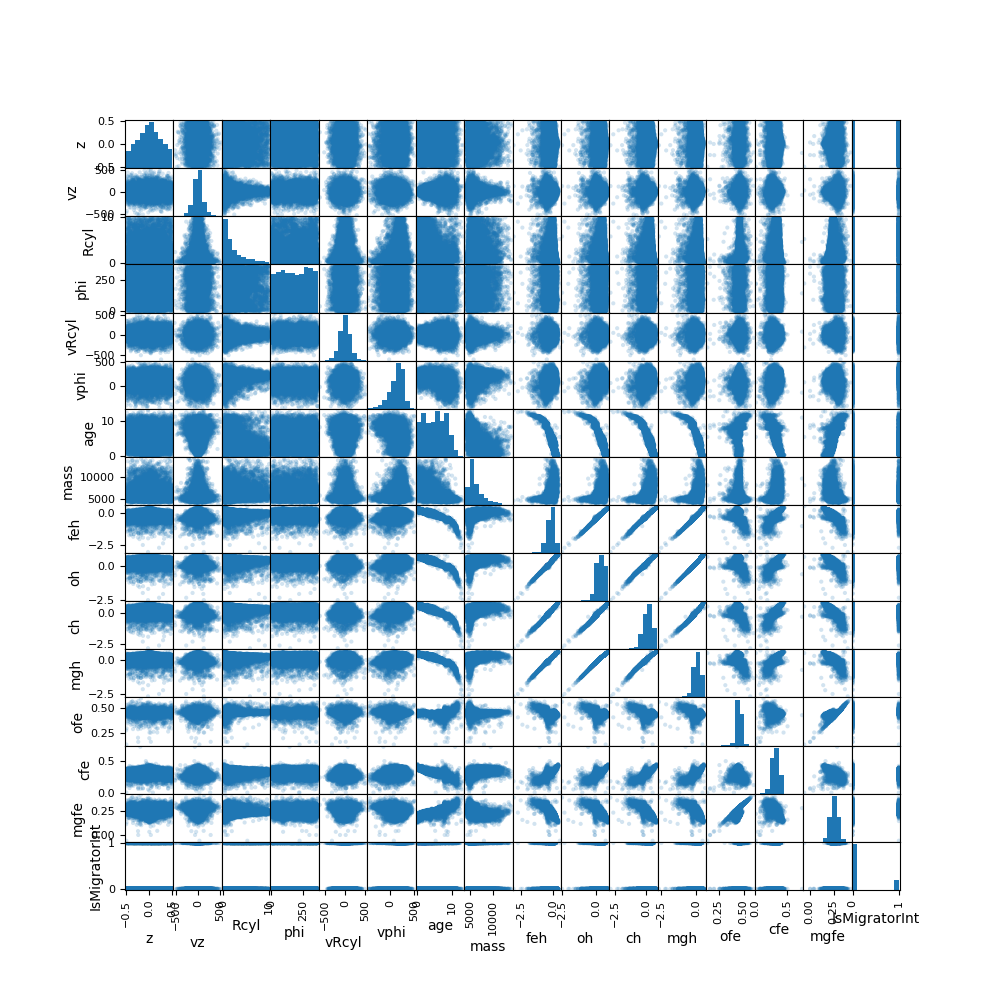
\includegraphics[width=\columnwidth]{Plots/scatter_matrix.png}
    \caption{Box plots of sample data}
    \label{fig:boxplots}
\end{figure}


\subsubsection{\label{sec:boxplots}Boxplots}


If we look at the boxplots in Figure \ref{fig:boxplots} we especially notice that $Rcyl$ is higher for Migrators, both 1st quartile, the mean and the 3rd quartile. We note these as important predictors, which we will also discover in later analysis. We observe the same for $vphi$, although it isn't as clear. Generally it seems that stars with extreme values of any predictor tends to be a migrator.


\subsubsection{\label{Clustering}Clustering analysis}
We start off by performing unsupervised learning in the form of clustering analysis on the data. As seen in Figure \ref{fig:dendogram}, we choose to cut at height 13. This leaves us with few clusters in varying in size, which might not be a bad thing, depending on the data. But, we get one very large cluster and few smaller. If we were to have chosen a smaller height, we would have many small clusters, perhapse too many. There is a tradeoff here of having large clusters, that don't really say much about the data, while too small clusters defeats the purpose of clustering (by e.g. having clusters with single data points.)



We don't really get anything exciting with our ratios (neither close to one or zero), not even at height 7, which  probably means that K nearest neighbors will not perform too well and that it in general might be difficult to categorize migrators with a model, since the stars seem to have the same attributes for both migrators and non-migrators.

\begin{figure}[h!]
    \centering
    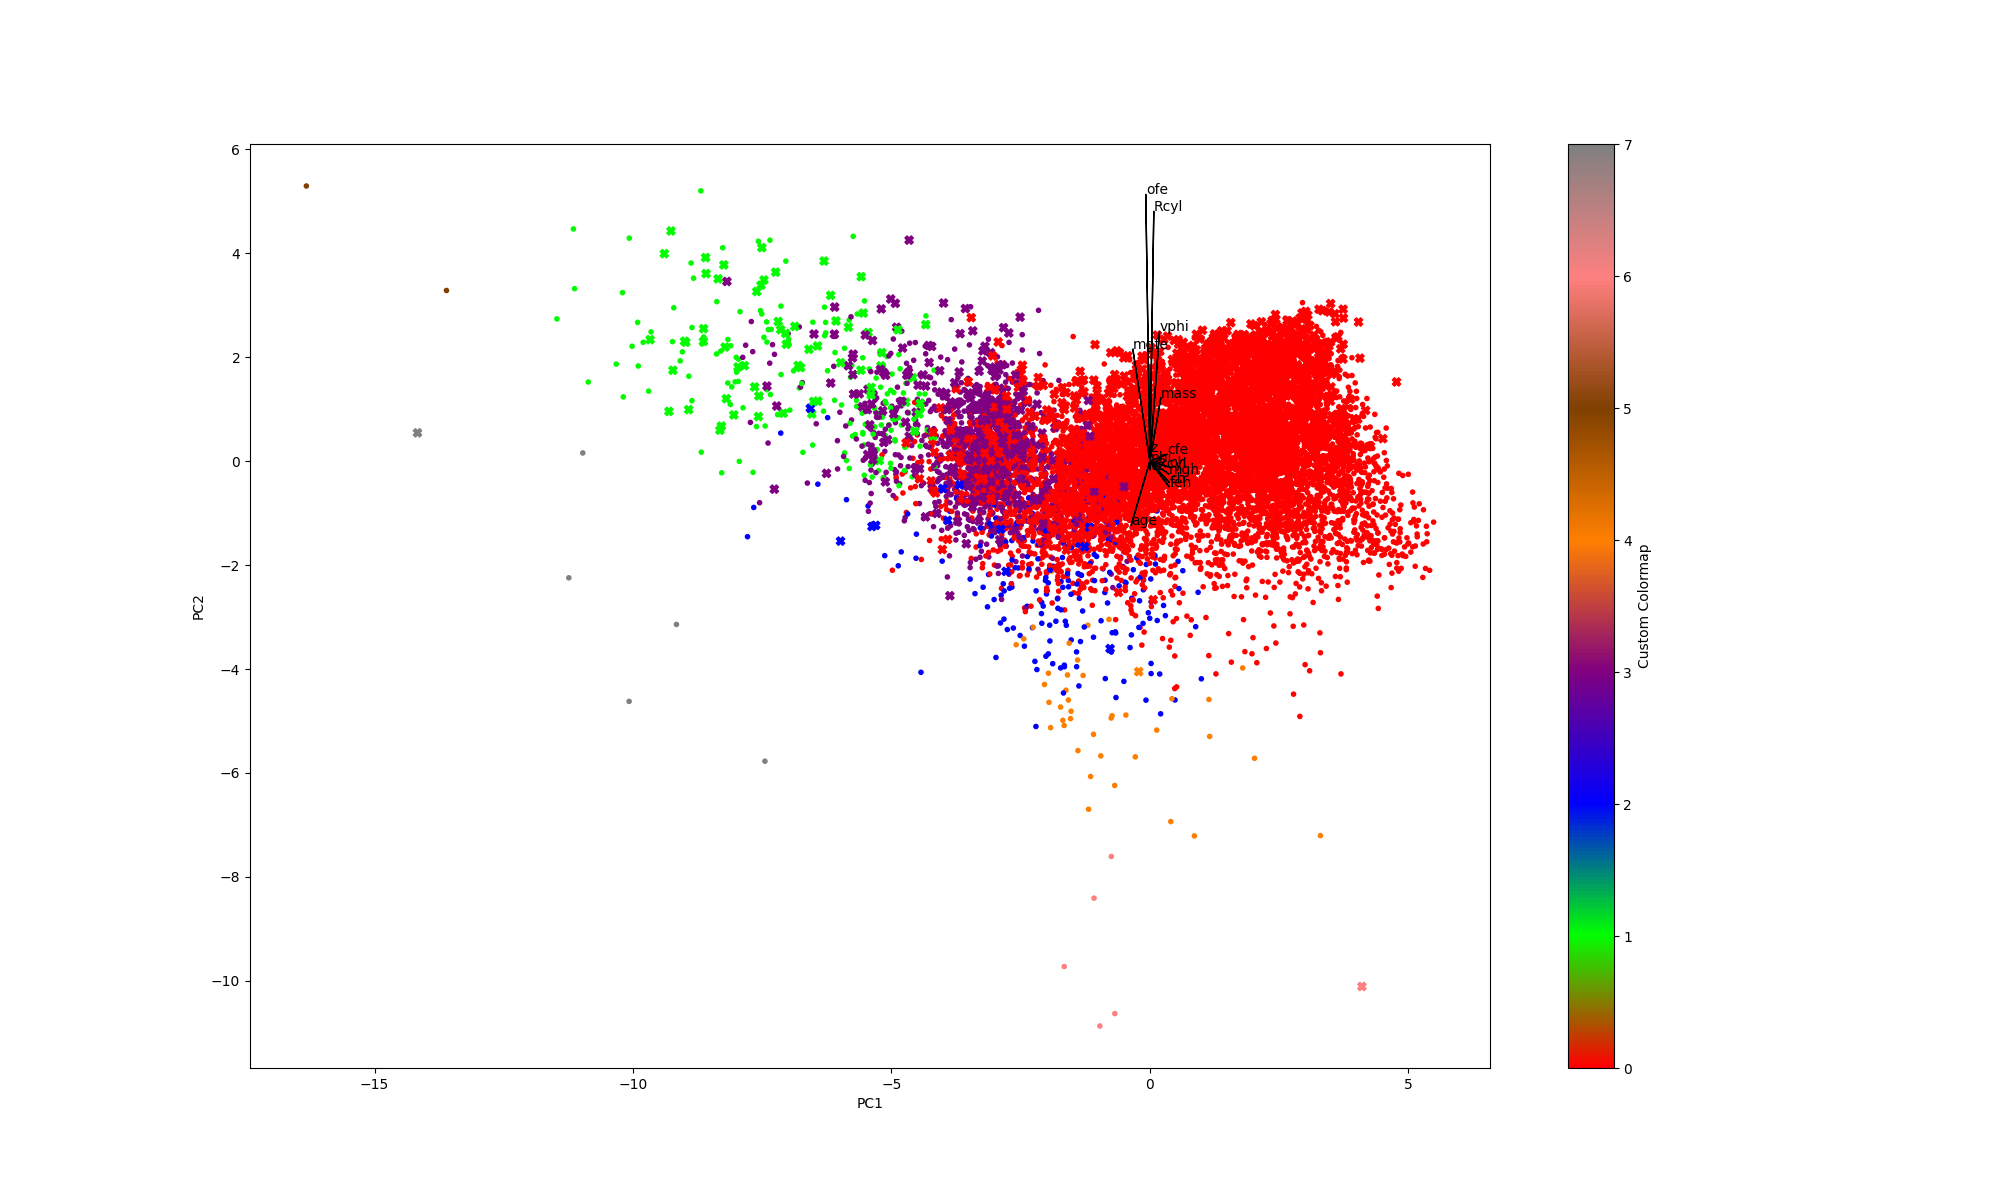
\includegraphics[width=\columnwidth]{Plots/Biplot_with_clustering.png}
    \caption{Scatter Matrix of sample data}
    \label{fig:biplot}
\end{figure}

Using dimensionality reduction does not yield great results either as seen in fig \ref{fig:biplot}, as the clusters don't have well defined lines in a 2d prediction, although this may be due to the high dimensionality data.
\begin{figure*}[t]
    \centering
    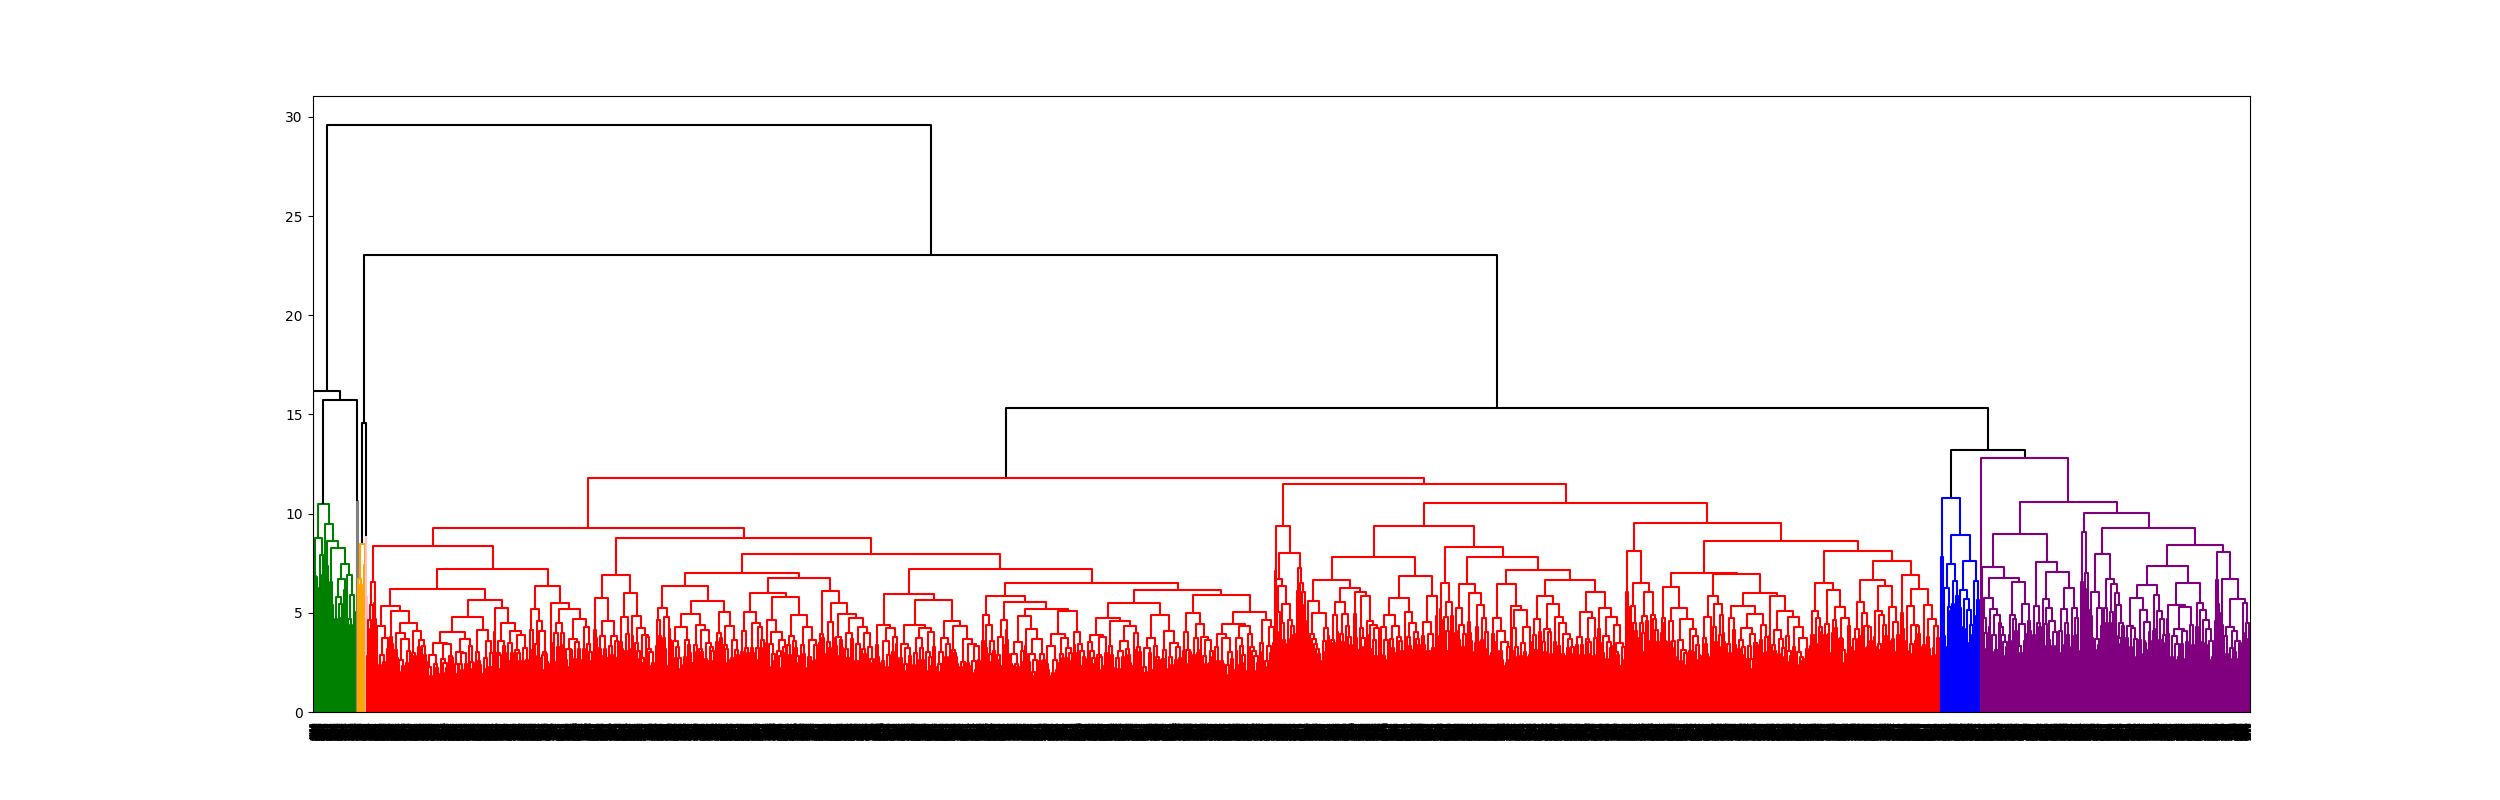
\includegraphics[width=\textwidth]{Plots/Dendrogram.png}
    \caption{Dendogram cut at height 13}
    \label{fig:dendogram}
\end{figure*}
\subsection{\label{sec:models}Models}
\subsubsection{\label{sec:GLM}Multiple Logistic Regression}
To reduce bias and variance in our model we use best subset selection, as we discussed in section \ref{sec_level1}. Looking at the results in table \ref{tab:BestSubset} we observe that the predictor $Rcyl$ gets added first, followed by $mgfe$/$ch$, $vphi$ and $age$. We already predicted that $Rcyl$ and $vphi$ were important predictors, and it makes sense that the model chooses almost randomly between the concentration predictors, since they are highly correlated.
\begin{table}[h!]
\caption{Best subset selection results for k predictors}
\label{tab:BestSubset}
\resizebox{\columnwidth}{!}{
\begin{tabular}{lrrrrrrrrrrrrrrr}
\toprule
 & Rcyl & age & cfe & ch & feh & intercept & mass & mgh & ofe & oh & phi & vRcyl & vphi & vz & z \\
\midrule
0 & - & - & - & - & - & -1.53 & - & - & - & - & - & - & - & - & - \\
1 & 0.48 & - & - & - & - & -3.09 & - & - & - & - & - & - & - & - & - \\
2 & 0.50 & - & -5.19 & - & - & -1.55 & - & - & - & - & - & - & - & - & - \\
3 & 0.48 & - & - & -1.20 & - & -3.57 & - & - & - & - & - & - & 0.00 & - & - \\
4 & 0.46 & - & -8.17 & - & - & -6.12 & - & - & 10.88 & - & - & - & 0.00 & - & - \\
5 & 0.40 & -0.34 & - & -13.69 & - & -0.88 & - & 12.86 & - & - & - & - & 0.00 & - & - \\
6 & 0.39 & -0.43 & - & -12.21 & - & 1.42 & - & 20.08 & - & -9.16 & - & - & 0.00 & - & - \\
7 & 0.39 & -0.44 & 7.09 & -16.67 & - & -0.47 & - & 24.66 & - & -9.32 & - & - & 0.00 & - & - \\
8 & 0.39 & -0.44 & 7.13 & -16.68 & - & -0.47 & - & 24.69 & - & -9.34 & - & - & 0.00 & - & 0.10 \\
9 & 0.39 & -0.44 & 7.19 & -16.67 & - & -0.48 & - & 24.72 & - & -9.39 & - & - & 0.00 & -0.00 & 0.09 \\
10 & 0.39 & -0.44 & - & -9.46 & 78.85 & -0.55 & - & 24.67 & 86.16 & -95.40 & - & - & 0.00 & -0.00 & 0.09 \\
11 & 0.39 & -0.44 & - & -9.49 & 80.23 & -0.48 & -0.00 & 24.34 & 87.48 & -96.41 & - & - & 0.00 & -0.00 & 0.09 \\
12 & 0.39 & -0.44 & -48.14 & 38.64 & 48.79 & -0.47 & -0.00 & 24.32 & 104.13 & -113.08 & - & - & 0.00 & -0.00 & 0.09 \\
13 & 0.39 & -0.44 & -49.49 & 40.04 & 47.26 & -0.70 & -0.00 & 24.17 & 103.99 & -112.78 & 0.00 & - & 0.00 & -0.00 & 0.08 \\
14 & 0.39 & -0.44 & -49.81 & 40.31 & 46.39 & -0.70 & -0.00 & 24.16 & 103.41 & -112.16 & 0.00 & -0.00 & 0.00 & -0.00 & 0.08 \\
\bottomrule
\end{tabular}
}
\end{table}


If we take a look at figure \ref{fig:BicAicAccuracy}
% \begin{figure}
%     \centering
%     \includegraphics[width=0.5\linewidth]{}
%     \caption{Caption}
%     \label{fig:enter-label}
% \end{figure}
we observe that the accuracy is highest for 10 predictors, but stays pretty much the same after adding $Rcyl$, where BIC is  at a minimum at 6 predictors and AIC keeps falling, but very little. This leads to the conclusion that the best number of predictors is 6. The accuracies are actually pretty low if you compare with the most naive classifier, which only predicts non-migrators, with an accuracy of 82,4\%, since the dataset is skewed towards non-migrators.

\begin{figure}[h!]
    \centering
    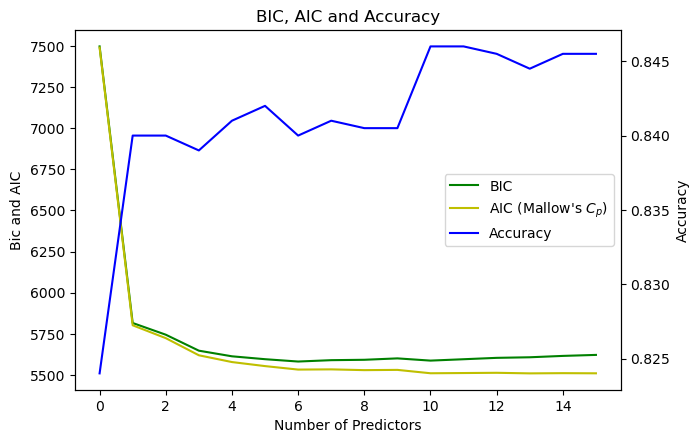
\includegraphics[width=0.8\columnwidth]{Plots/BIC, AIC, ACC all 15.png}
    \caption{BIC, AIC and Accuracy as a function of number of predictors in best subset selection}
    \label{fig:BicAicAccuracy}
\end{figure}

% We then perform logistic regression on the full dataset, both using all of the predictors and yielding an accuracy of 83.1\% and only using the predictors found in best subset selection yielding an accuracy of 82,3\%, which curiously is lower than that of the most naive classifier that only predicts non-migrators, with an accuracy of 82,4\%. Both are actually lower than what we see from the models trained on sampled data, although this performance drop is likely due to not removing outliers from the full dataset and generally we can conclude that logistic regression is not a good fit for predicting migrators.
\subsubsection{\label{sec:KNN}K Nearest Neighbors}


We performed a K Nearest Neighbor for $K\in[0,150]$ to see how it performed.
% \begin{figure}
%     \centering
%     \includegraphics[width=0.5\linewidth]{}
%     \caption{Caption}
%     \label{fig:enter-label}
% \end{figure}
As seen in figure \ref{fig:KNN} KNN performs best at $K=6$ with an accuracy of 84.2\%, which is not our best performing model, but slightly better than the most naive classifier.

\begin{figure}[h!]
    \centering
    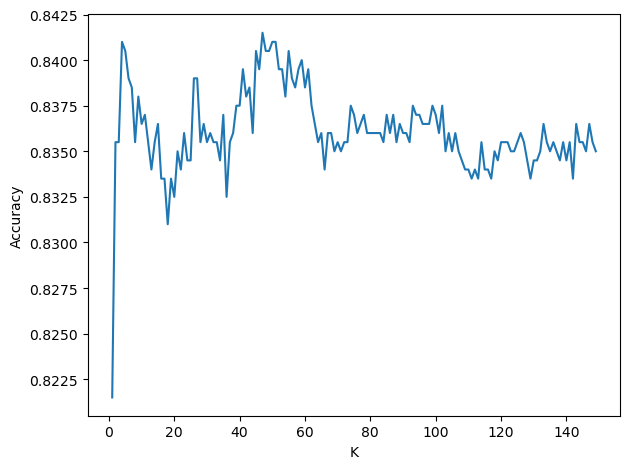
\includegraphics[width=0.8\columnwidth]{Plots/KNN_150accuracy.png}
    \caption{Box plots of sample data}
    \label{fig:KNN}
\end{figure}
\subsubsection{\label{sec:Trees}Tree Based Methods}
First start off simply by using cost complexity pruning where we tune the pruning paramater $\alpha$ by 10-fold cross-validation, which yields the tree in figure \ref{fig:DecisionTree} and a test accuracy of 82.9\%, which is lower than that of the most naive model, altough we again do conforim or hypothesis that $Rcyl$ and $vphi$ are important predictors.

Our tree-based models performed pretty similar, all with an accuracy that rounds to 87\%.

First we performed bagging using sklearns RandomForestClassifier and achieve a test accuracy of 86.8\%, where the predictors of highest importance $Rcyl$, $v\phi$ and $vRcyl$. We use this model to investigate our decision boundary in fig. \ref{fig:ratevsdb} and it seems that 0.5 is a really good threshold, since the sensitivity and precision curves cross at $T\approx0.5$. We also plot an ROC-curve in figure \ref{fig:ROC}, where the $AUC>0.5$ and our model is definitely better than chance.


\begin{figure}[h!]
    \centering
    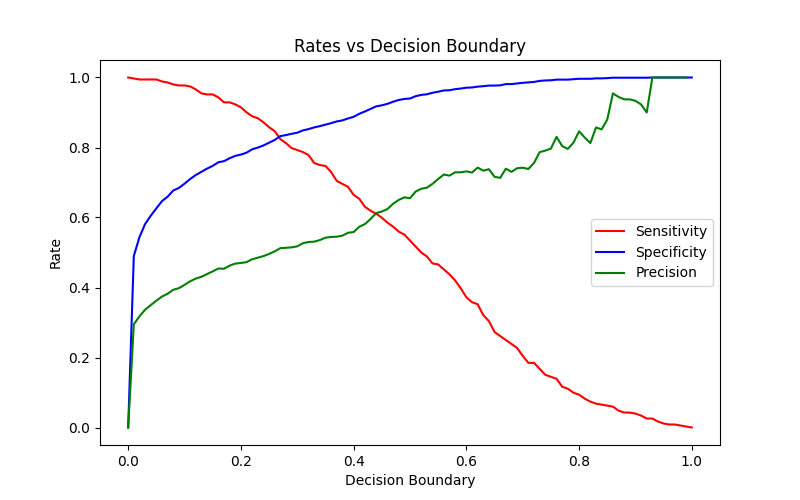
\includegraphics[width=0.75\columnwidth]{Plots/Rates_vs_DecisionBoundary.png}
    \caption{}
    \label{fig:ratevsdb}
\end{figure}

\begin{figure}[h!]
    \centering
    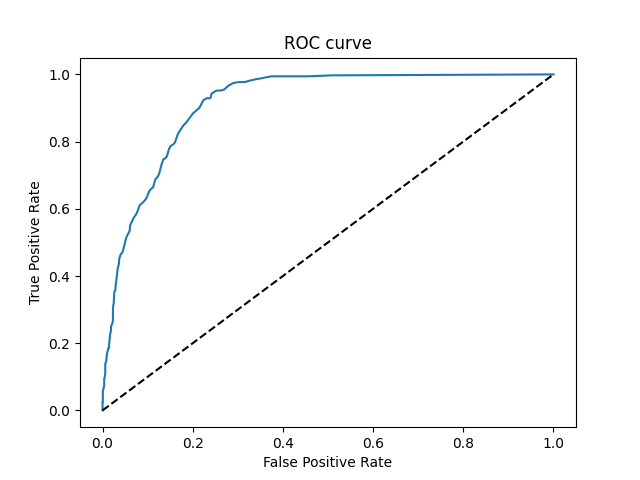
\includegraphics[width=0.8\columnwidth]{Plots/ROC_curve.png}
    \caption{}
    \label{fig:ROC}
\end{figure}
\newpage

We then perform random forrest for a range of maximum features in figure \ref{fig:randomforrest}. We noticed that our accuracy jumped quite a lot (within a small range), so we repeated the experiment for multiple random states, and the fluctuations seem to be due to random chance. The best performing models peak over 87\% and we cannot determine a best number of features, although it is probably more than 5.


\begin{figure}[h!]
    \centering
    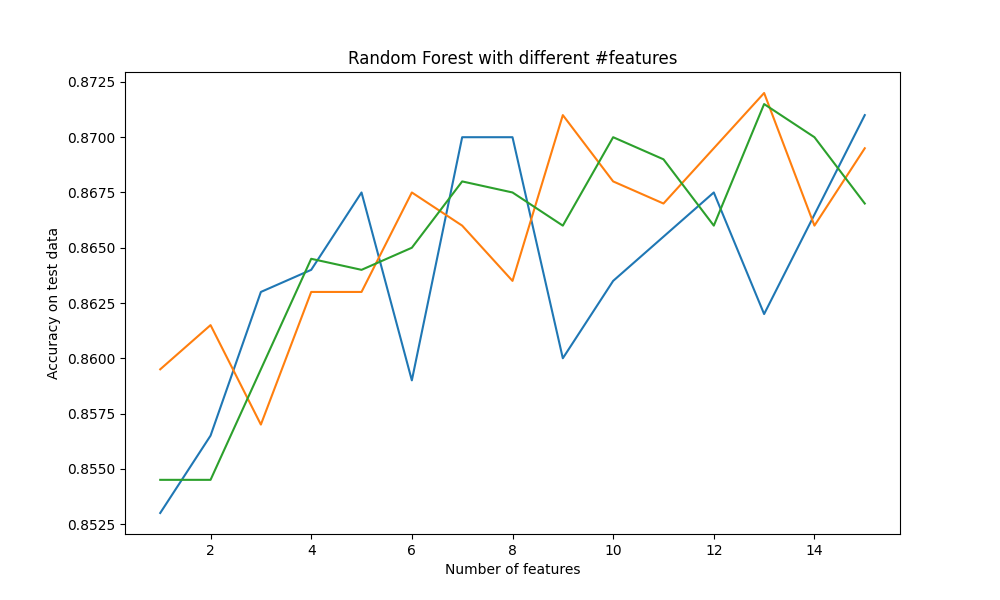
\includegraphics[width=0.75\columnwidth]{Plots/RandomForest.png}
    \caption{}
    \label{fig:randomforrest}
\end{figure}


At last we performed boosting. We trained 1000 trees with a maximum depth of 3 and variety shrinkage parameters $\lambda$, although the best performing one was with $\lambda = 0.01$, where we achieved a testing accuracy of 87.4\%. As seen in figure \ref{fig:accuracyvslambda} the accuracy shrinks for higher values of $\lambda$, which is just a sanity check, since the model is fine tuned more and more for smaller $\lambda$.


\begin{figure}[h!]
    \centering
    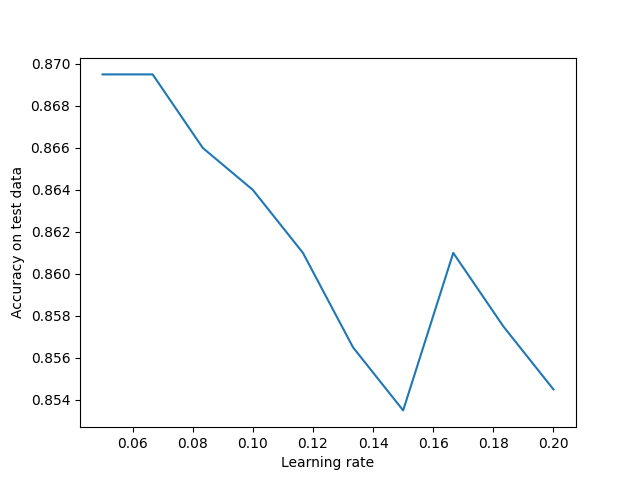
\includegraphics[width=0.75\columnwidth]{Plots/GradientBoosting.png}
    \caption{Gradient Boosting accuracy for different learning rates, $\lambda$}
    \label{fig:accuracyvslambda}
\end{figure}


In general the tree-based methods perform well compared to our other models, which is probable due to the fact that the trees are flexible enough to catch the small details, while keeping the variance down from taking the average.
\subsubsection{\label{sec:NN}Neural Networks}
As a final type of model, we tried using neural networks. The best performing one, was a simple neural network trained on the full dataset, having one dense layer of 16 neurons using the relu activation function and an output-layer of one neuron, using the sigmoid activation function to get a probability of the star being a migrator. It was trained using cross entropy as the loss-function and adam as the optimizer. Here we achieved an accuracy of 88\%, called Neural Network 5 in table \ref{tab:RawData}. The rest of the Neural Networks were only trained on the sample data.
\begin{table}[h!]
\caption{Differnet neural networks}
\label{tab:RawData}
\resizebox{\columnwidth}{!}{
\begin{tabular}{llllrrlrlrr}
\toprule
 &  & Optimizer & Loss & Accuracy & Layer # & Layer Type & Neurons & Activation & epochs & Rate \\
\midrule
\multirow[t]{3}{*}{Neural Network 1} & 0 & adam & binary\textunderscore crossentropy & 0.851 & 1 & Dense & 64.000 & relu & 100 & - \\
 & 1 & adam & binary\textunderscore crossentropy & 0.851 & 2 & Dense & 64.000 & relu & 100 & - \\
 & 2 & adam & binary\textunderscore crossentropy & 0.851 & 3 & Dense & 1.000 & sigmoid & 100 & - \\
\cline{1-11}
\multirow[t]{3}{*}{Neural Network 2} & 3 & adam & categorical\textunderscore crossentropy & 0.847 & 1 & Dense & 64.000 & relu & 100 & - \\
 & 4 & adam & categorical\textunderscore crossentropy & 0.847 & 2 & Dense & 64.000 & relu & 100 & - \\
 & 5 & adam & categorical\textunderscore crossentropy & 0.847 & 3 & Dense & 2.000 & softmax & 100 & - \\
\cline{1-11}
\multirow[t]{2}{*}{Neural Network 3} & 6 & adam & binary\textunderscore crossentropy & 0.866 & 1 & Dense & 16.000 & relu & 100 & - \\
 & 7 & adam & binary\textunderscore crossentropy & 0.866 & 2 & Dense & 1.000 & sigmoid & 100 & - \\
\cline{1-11}
\multirow[t]{5}{*}{Neural Network 4} & 8 & adam & binary\textunderscore crossentropy & 0.847 & 1 & Dense & 16.000 & relu & 100 & - \\
 & 9 & adam & binary\textunderscore crossentropy & 0.847 & 2 & Dropout & - & - & 100 & 0.500 \\
 & 10 & adam & binary\textunderscore crossentropy & 0.847 & 3 & Dense & 16.000 & relu & 100 & - \\
 & 11 & adam & binary\textunderscore crossentropy & 0.847 & 4 & Dropout & - & - & 100 & 0.500 \\
 & 12 & adam & binary\textunderscore crossentropy & 0.847 & 5 & Dense & 1.000 & sigmoid & 100 & - \\
\cline{1-11}
\multirow[t]{2}{*}{Neural Network 5} & 13 & rmsprop & binary\textunderscore crossentropy & 0.880 & 1 & Dense & 16.000 & relu & 10 & - \\
 & 14 & rmsprop & binary\textunderscore crossentropy & 0.880 & 2 & Dense & 1.000 & sigmoid & 10 & - \\
\cline{1-11}
\bottomrule
\end{tabular}
}
\end{table}

Of the models only trained on sample data we observe that it is actually the simplest model with only one dense layer with 16 neurons, that performs the best, Neural Network 3, which is why we chose to train a similar neural network on all of the data. It is clear that adding more neurons decreases the testing performance of the model, likely due to overfitting, while it is unclear whether more layers increases or decreases the testing accuracy. It is also worth noting, that using either sigmoid or softmax performs the same.

\section{DISCUSSION}
The models are not that far from the baseline of a model always guessing nomigrator. It seems it is very difficult to classify stars as migrators and it may be far more determined by other factors, such as how dense it's local environment is (or rather was), proximity to black holes etc. than the variables we accounted for in this study. 

A key factor to notice in our models is the fact that it is trained using simulation data, and we will never know how accurate our models really are on real world data, since it's impossible to measure migration of stars on our timescale. This will purely be a statistical tool that can point us in different directions for further study. It may even be possible that we are just fitting our models to simulation errors and that the predictions are completely unusable in the field.

Further study would be growing forests using all of the data and perhaps trying deeper layered neural networks, while keeping the amount of neurons per layer fairly low. Also training for a larger amount of epochs would help, and different optimizers could be tried. As goes for the tree based methods, training them on the full dataset would be a great start.


\section{CONCLUSION}
In conclusion, we have effectively creates models that are able to predict whether og not a star could be classified as a migrator. The best performing model was a pretty simpe neural network, consisting of a dense layer of 16 neurons, with a test accuracy of 88\%. This type of model, was the best performing of the models we ran on the sample data, which is why it was chosen to be trained on the full dataset.
The tree-based methods all performed well, achieving accuarcies around 87\% (depending on the specific model you choose), which is likely due to them being very flexible, while taking the mean result keeps the variance down. The performance of the models are only slightly higher than that of the most naive classifier, which has an accuracy of 82,4\% on the testing data. This is likely due to the fact that migration of stars is dependent on other factors, which probably are local to the formation place of the stars and therefore non-predictable from current data. It is also worth noticing that our models are trained on simulation data and may not, although unlikely, be unusable in the field. They should be seen as a statistical tool, to point researchers in different directions. They could be improved by trying even more different models and training the models on the full dataset.

\newpage

\nocite{*}
\section*{\underline{Citations}}
\bibliography{aapmsamp}% Produces the bibliography via BibTeX.


\appendix \section{Extra plots} % \input{Python}
 
\begin{figure}[h!]
    \centering
    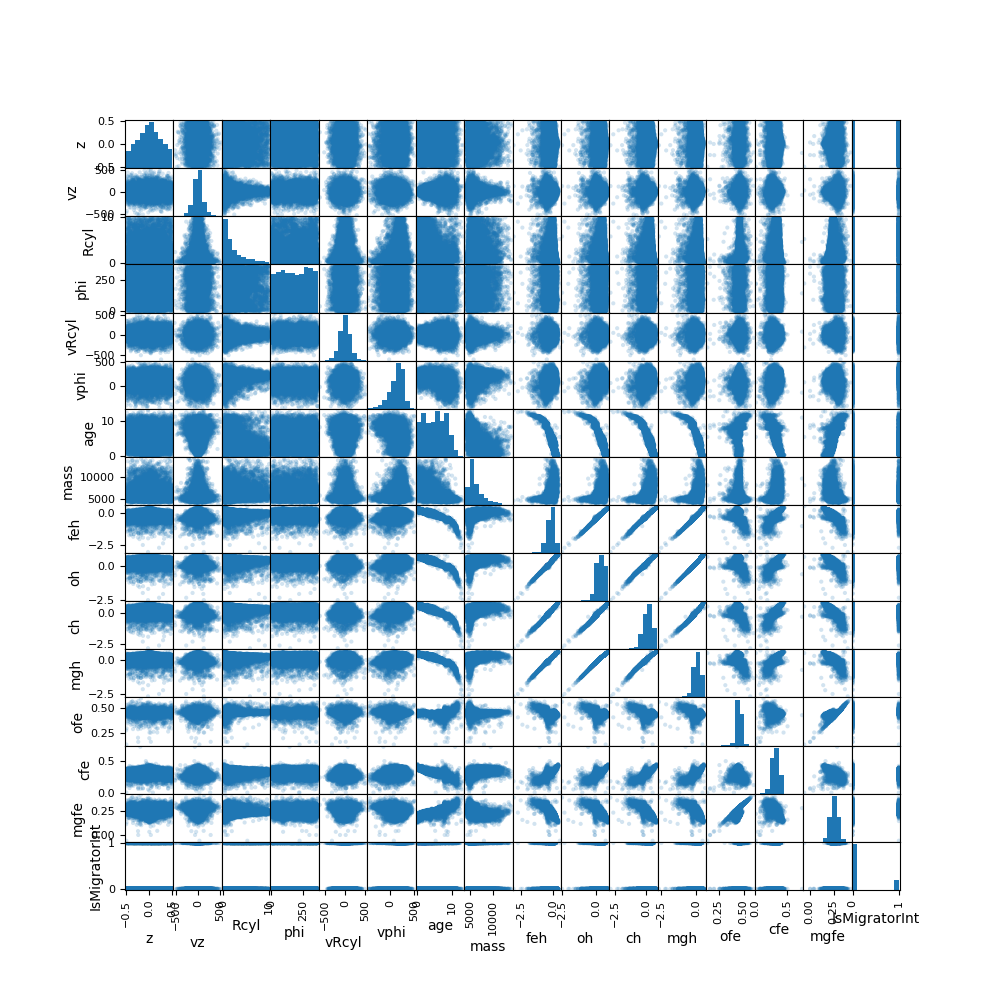
\includegraphics[width=\columnwidth]{Plots/scatter_matrix.png}
    \caption{Scatter Matrix of sample data}
    \label{fig:scattermatrix}
\end{figure}


\begin{figure}[h!]
    \centering
    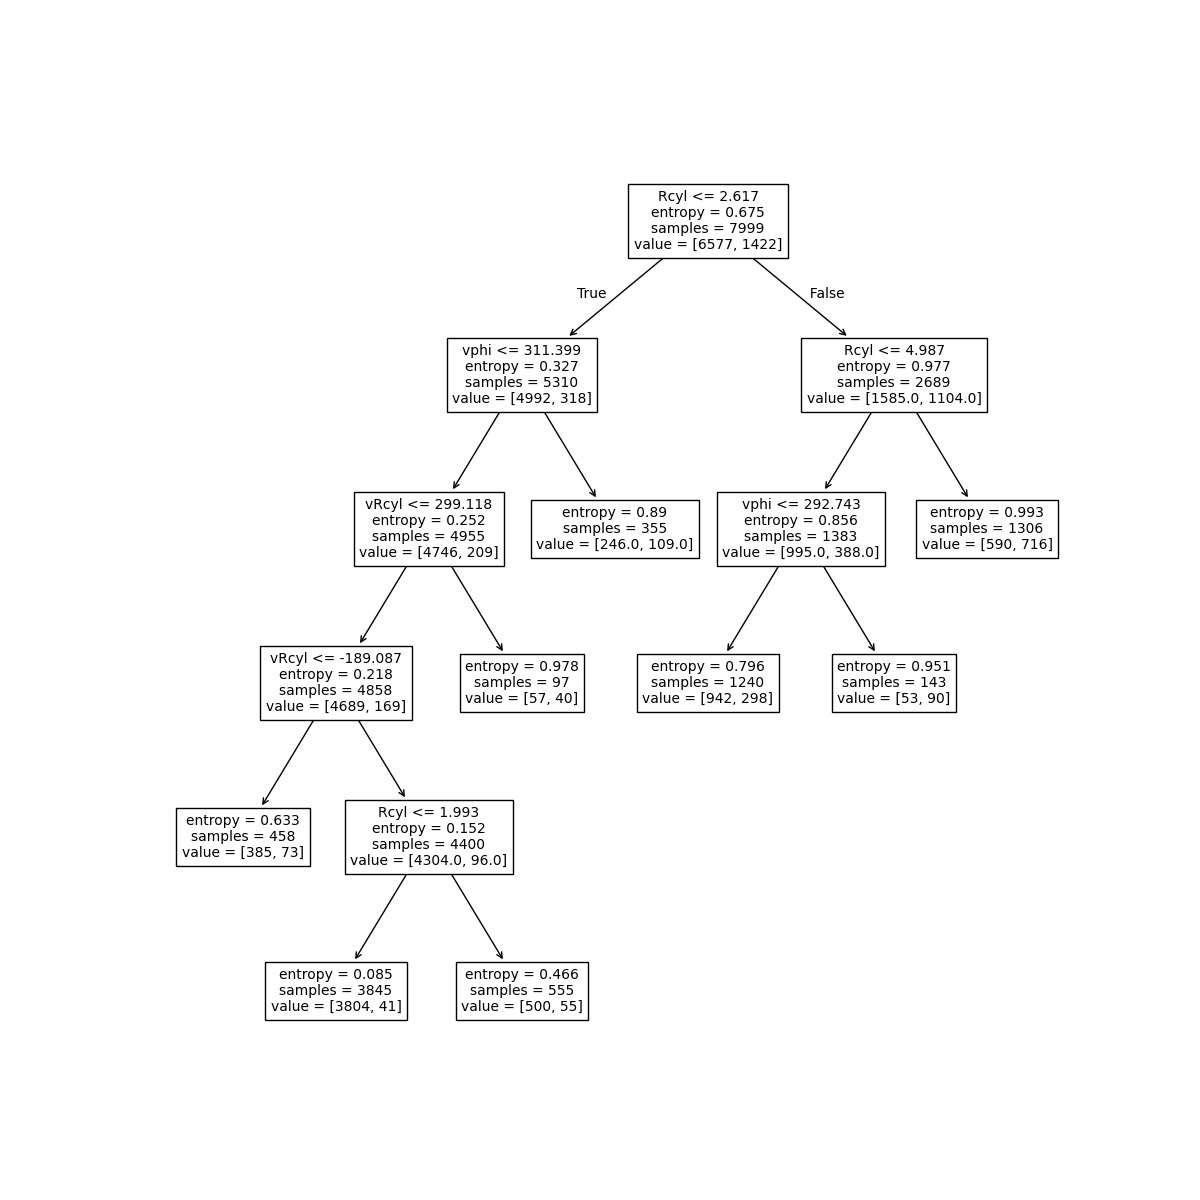
\includegraphics[width=\columnwidth]{Plots/DecisionTree.png}
    \caption{Decision tree of a pruned tree}
    \label{fig:DecisionTree}
\end{figure}




\end{document}
%
% ****** End of file aapmsamp.tex ******
